\documentclass{aa}		% two-column
% \documentclass[referee]{aa}		% referee one-column
\usepackage[english]{babel}
\usepackage[utf8]{inputenc}
\usepackage{amsmath,amsfonts,amssymb,enumerate}
\usepackage{txfonts,graphics,graphicx,epstopdf,float,lscape,longtable,dcolumn,footnote,subcaption,caption,color,url,hyperref,listings,esvect}
\usepackage{rotating,afterpage}

% Added by Juan
\usepackage{soul,xcolor}
\newcommand{\jcim}[1]{\textbf{\textcolor{green}{#1}}}
\newcommand{\mm}[1]{\textbf{\textcolor{purple}{#1}}}
\newcommand{\rc}[1]{\textbf{\textcolor{red}{#1}}}
\newcommand{\thh}[1]{\textbf{\textcolor{blue}{#1}}}

\setstcolor{red}  
\newcommand{\stjc}[1]{\st{#1}}


\newenvironment{amssidewaysfigure}
	{\begin{sidewaysfigure}\vspace*{.75\textwidth}\begin{minipage}{\textheight}\centering}{\end{minipage}\end{sidewaysfigure}}
\newenvironment{mysidewaysfigure}
	{\begin{sidewaysfigure*}\vspace*{.75\textwidth}\centering}{\end{sidewaysfigure*}}
\newcommand*\xbar[1]{{\hbox{\vbox{\hrule height 0.5pt \kern0.5ex \hbox{\kern-0.1em \ensuremath{#1} \kern-0.1em}}}}}

\usepackage{natbib}
	\bibpunct{(}{)}{;}{a}{}{,} % to follow the A&A style

\defcitealias{IbanezMejia2016}{Paper I}
\defcitealias{IbanezMejia2017}{Paper II}
\defcitealias{Chira2018}{Paper III}

%  Abbreviations
% For ptex, put in \ts for thin space, latex \,
\newcommand{\longpage}{\enlargethispage{\baselineskip}}
\newcommand{\shortpage}{\enlargethispage{-\baselineskip}}
\newcommand{\veryshortpage}{\enlargethispage{-2\baselineskip}}
%\newcommand{\text}{\textrm}
\def\Lsun {\hbox{$L_\odot$}}
\def\Msun {\hbox{$M_\odot$}}
\def\ts {\thinspace}
\def\etal {et al.}
\def\ie {i.\, e.}
\def\etseq {{\it et seq.}}
\def\vs {{it vs.}}
\def\perse {{it per se}}
\def\adhoc {{\it ad hoc}}
\def\eg {e.g.}
\def\etc {etc.}
\def\ER {$\pm $}   % Plus-minus
\def\vtwo  {v$_2$}
\def\ccpers {\hbox{${\rm cm}^3{\rm s}^{-1}$}}
\def\TVIB {\hbox{$T_{\rm vib}$}}
\def\TROT {\hbox{$T_{\rm rot}$}}
\def\TVIBST {T${\rm vib}^*$}
\def\TEXC {\hbox{$T_{\rm ex}$}}   % Tex
\def\TONT {\hbox{${\rm T}_{12}$}}   %T12 between (1,1) and (2,2)
\def\DBYDV {\hbox{${\rm d}_{*}/\Delta {\rm v}$}}
\def\TKIN {\hbox{$T_{\rm kin}$}}      %   Tkin
\def\TEX {\hbox{$T_{\rm ex}$}}      %   Tex
\def\TMB {\hbox{$T_{\rm MB}$}}      %   Tmb
\def\ra {& \rightarrow &}
\def\rla {& \rightleftharpoon &}
\def\J {$J$}
%
\def\apj{{Astrophys. J.} }
\def\apjl{{Astrophys. J. Lett.} }
\def\asj{{Astron. J.}}
\def\aua{{Astron. Astrophys.} }
\def\aap{{Astron. Astrophys.} }
\def\mnras{{Monthly Notices Roy. Astron. Soc.} }
\def\araa{{Ann. Rev. Astron. Astrophys.} }
\def\comma{{Comments on Astrophys.} }
\def\AAREV{{The Astron. and Astrophys. Review}}
\def\JQuanSRT {{J. Quant. Spectrosc. Rad. Transf.}}
\def\apjs {{Astrophys. J. Suppl.}}
\def\apjsupp {{Astrophys. J. Suppl.}}
\def\AASupp {{Astron. Astrophys. Suppl.}}
\def\AlComm {{Astroph. Lett. and Comm.}}
\def\PhysRev {{Phys. Rev.}}
\def\pasp {{The Publ. of the Astron. Soc. of the Pacific}}
\def\pre {{Phys. Rev. E.}}
\def\PhRLett {{Phys. Rev. Lett.}}
\def\JPCREF {{J.Phys.Chem.Ref.Data}}
\def\JCHEMPH {{J. Chem. Phys.}}
\def\JMOLSP {{J. Molec. Spectrosc.}}
\def\RevMP {{Rev. Mod. Phys.}}
\def\science {{Science}}
\def\ICARUS {{Icarus}}
\def\nat {{Nature}}
\def\nature {{Nature}}

\def\vlsr {$v_{\rm lsr}$}
\def\AU {{\footnotesize AU}}
\def\mic {$\mu\hbox{m}$}
\def\solmass {\hbox{$M_\odot$}}
\def\solum {$\hbox{L}_\odot$}
\def\rhounit {$\hbox{M}_\odot\, \hbox{pc}^{-3}$}
\def\kms {\hbox{${\rm km\, s}^{-1}$}}
\def\pers {\hbox{${\rm s}^{-1}$}}
\def\kmsL {\hbox{${\rm km\, s}^{-1}$}}
\def\percc {\hbox{{\rm cm}$^{-3}$}}    %cm-3
\def\cmsq  {\hbox{{\rm cm}$^{-2}$}}    %cm-2
\def\cmsix  {\hbox{{\rm cm}$^{-6}$}}  %cm-6
\def\h {\hbox{$^{\rm h}$}}
\def\m {\hbox{$^{\rm m}$}}
\def\arcsec {\hbox{$^{\prime\prime}$}}
\def\arcmin {\hbox{$^{\prime}$}}
\def\HI  {\hbox{H{\sc i}}}
\def\HII  {\hbox{H{\sc ii}}}
\def\HeII  {\hbox{He{\sc ii}}}
\def\UCHII  {\hbox{UCH{\sc ii}}}
\def\CI {\hbox{C{\sc i}}}
\def\CII {\hbox{C{\sc ii}}}
\def\SiII {\hbox{Si{\sc ii}}}
\def\OI {\hbox{O{\sc i}}}
\def\OIII {\hbox{O{\sc iii}}}
\def\NeII {\hbox{Ne{\sc ii}}}
\def\NII {\hbox{N{\sc ii}}}
\def\NIII {\hbox{N{\sc iii}}}
\def\sigdust {\hbox{$\overline{\sigma _{g}}$}} % Mean grain cross sec/H
\def\vtwo {\hbox{v$_2$}}
\def\erg {\hbox{${\rm erg\ cm}^{-2} {\rm s}^{-1} {\rm sr}^{-1}$}}
\def \AV {\hbox{$A_{\rm V}$}}
%
%   Abbreviations for radio recomb lines etc
 \def \AL {$\alpha $}     %  gr. alpha
 \def \BE {$\beta $}     % gr. beta
 \def \GA {$\gamma $}    % gr. gamma
 \def \DE {$\delta $}    % gr. delta
 \def \EP {$\epsilon $}  % gr. epsilon
\def \si {$\sigma $}
\def \BN  {\hbox{${\rm b}_n$}} %    bn
 \def \BETAN {\hbox{$\beta _n$}} %  beta factor
 \def \TE {\hbox{${\rm T}_{\rm e}$}}  % Electron Temp.
 \def \TELTE {\hbox{${\rm T}_{\rm e}^{*}$}} % LTE Electron Temp.
 \def \NE {\hbox{${\rm N}_{\rm e}$}}  % Electron Dens.
 \def \YPLUS {\hbox{${\rm Y}^{+}$}}   %  He+/H+ ratio
 \def \HEHRAT {\hbox{${\rm He}^{+}/{\rm H}^{+}$}}
% molecules
%
\typeout{loading alias}
\def\e    {\hbox{\rm e}}     % e
\def\H    {\hbox{\rm H}}     % H
\def\OX   {\hbox{\rm O}}     % O
\def\N    {\hbox{\rm N}}     % N
\def\M    {\hbox{\rm M}}     % M
\def\A    {\hbox{A}}     % A
\def\APL    {\hbox{\rm A$^+$}}     % A+
\def\AP    {\hbox{$A^+$}}     % A+
\def\AM    {\hbox{$A^-$}}     % A-
\def\APLUS    {\hbox{$A^+$}}     % A+
\def\AMINUS    {\hbox{$A^-$}}     % A-
\def\APM    {\hbox{$A^\pm$}}     % A+/-
\def\AMP    {\hbox{$A^\mp$}}     % A-/+
\def\E    {\hbox{$E$}}     % E
%\def\AA    {\hbox{$AA$}}     % AA  % conflicts with Angstrom
\def\EE    {\hbox{$EE$}}     % EE
\def\EA    {\hbox{$EA$}}     % EA
\def\AE    {\hbox{$AE$}}     % AE
\def\B    {\hbox{\rm B}}     % B
\def\BPL    {\hbox{\rm B$^+$}}     % B+
\def\C    {\hbox{\rm C}}     % C
\def\D    {\hbox{\rm D}}     % D
\def\halpha {\hbox{\rm H$\alpha $}}     % Halpha
\def\AB    {\hbox{\rm AB}}     % AB
\def\BC    {\hbox{\rm BC}}     % BC
\def\ABPL    {\hbox{\rm AB$^+$}}     % AB+
\def\K    {\hbox{\rm K}}     % K
\def\CS   {\hbox{\rm CS}}    % CO
\def\SiO   {\hbox{\rm SiO}}    % CO
\def\CO   {\hbox{\rm CO}}    % CO
\def\COTW   {\hbox{\rm CO$_2$}}    % CO2
\def\NO   {\hbox{\rm NO}}    % NO
\def\OH   {\hbox{\rm OH}}    % OH
\def\NH   {\hbox{\rm NH}}    % NH
\def\HD   {\hbox{\rm HD}}    % HD
\def\NHTW {\hbox{\rm NH$_2$}}    % NH2
\def\NTW {\hbox{\rm N$_2$}}    % N2
\def\HTW {\hbox{\rm H$_2$}}    % H2
\def\CTW {\hbox{\rm C$_2$}}    % C2
\def\OTW {\hbox{\rm O$_2$}}    % O2
\def\HCN  {\hbox{\rm HCN}}   % HCN
\def\HNC  {\hbox{\rm HNC}}   % HNC
\def\DCN  {\hbox{\rm DCN}}   % DCN
\def\DNC  {\hbox{\rm DNC}}   % DNC
\def\CN  {\hbox{\rm CN}}     % CN
\def\CRP  {\hbox{\rm crp}}     % crp
\def\MOLH {\hbox{${\rm H}_2$}}  %H2
\def\MOLO {\hbox{${\rm O}_2$}}  %O2
\def\HDO {\hbox{${\rm HDO}$}}  %HDO
\def\NHTH {\hbox{${\rm NH}_{3}$}} %NH3
\def\AMM {\hbox{${\rm NH}_{3}$}} %NH3
\def\NHTWD {\hbox{${\rm NH}_2{\rm D}$}} %NH2D
\def\FAMM {\hbox{$^{15}{\rm NH}_{3}$}}  %15NH3
\def\CTWH {\hbox{${\rm C_{2}H}$}}  %C2H
\def\CTWHD {\hbox{${\rm C_{2}HD}$}}  %C2HD
\def\TWCO {\hbox{${\rm ^{12}CO}$}}  % 12CO
\def\TWC {\hbox{${\rm ^{12}C}$}}  % 12C
\def\THC {\hbox{${\rm ^{13}C}$}}  % 13C
\def\SIXO {\hbox{${\rm ^{16}O}$}}  % 16O
\def\SEO {\hbox{${\rm ^{17}O}$}}  % 17O
\def\EIO {\hbox{${\rm ^{18}O}$}}  % 18O
\def\THTWS {\hbox{${\rm ^{32}S}$}}  % 32S
\def\THTHS {\hbox{${\rm ^{33}S}$}}  % 33S
\def\THFOS {\hbox{${\rm ^{34}S}$}}  % 34S
\def\FON {\hbox{${\rm ^{14}N}$}}  % 14N
\def\FIN {\hbox{${\rm ^{15}N}$}}  % 15N
\def\TWESI {\hbox{${\rm ^{28}Si}$}}  % 28Si
\def\TWNSI {\hbox{${\rm ^{29}Si}$}}  % 29Si
\def\THSI {\hbox{${\rm ^{30}Si}$}}  % 30Si
\def\CEIO {\hbox{${\rm C}^{18}{\rm O}$}}   %C18O
\def\CSEO {\hbox{${\rm C}^{17}{\rm O}$}}   %C17O
\def\OCTHFOS {\hbox{${\rm OC}^{34}{\rm S}$}} % OC34S
\def\OTHCS {\hbox{${\rm O}^{13}{\rm CS}$}} % O13CS
\def\CTHFOS {\hbox{${\rm C}^{34}{\rm S}$}} % C34S
\def\CTHTWS {\hbox{${\rm C}^{32}{\rm S}$}} % C32S
\def\CTHTHS {\hbox{${\rm C}^{33}{\rm S}$}} % C33S
\def\TWEISIO {\hbox{$^{28}{\rm SiO}$}} % 28sio
\def\TWNISIO {\hbox{$^{29}{\rm SiO}$}} % 29sio
\def\THSIO {\hbox{$^{30}{\rm SiO}$}} % 30sio
\def\THCO {\hbox{$^{13}{\rm CO}$}}   %13CO
\def\TWCS {\hbox{$^{12}{\rm CS}$}}   %12CS
\def\THCS {\hbox{$^{13}{\rm CS}$}}   %13CS
\def\COT {\hbox{${\rm CO}_2$}}        %CO2
\def\WAT {\hbox{${\rm H}_2{\rm O}$}}   %H2O
\def\HTWO {\hbox{${\rm H}_2{\rm O}$}}   %H2O
\def\WATEI {\hbox{${\rm H}_2^{18}{\rm O}$}}   %H218O
\def\HTWEIO {\hbox{${\rm H}_2^{18}{\rm O}$}}   %H218O
\def\WATSE {\hbox{${\rm H}_2^{17}{\rm O}$}}  %H217O
\def\HTWSEO {\hbox{${\rm H}_2^{17}{\rm O}$}}  %H217O
\def\HTWS  {\hbox{${\rm H}_2{\rm S}$}}            % H2S
\def\HTHFOTWS  {\hbox{${\rm H}_2^{34}{\rm S}$}}            % H2S
\def\THTWSO  {\hbox{$^{32}{\rm SO}$}}            % 32SO
\def\THTHSO  {\hbox{$^{33}{\rm SO}$}}            % 33SO
\def\THFOSO  {\hbox{$^{34}{\rm SO}$}}            % 34SO
\def\SEIO  {\hbox{${\rm S}^{18}{\rm O}$}}            % S18O
\def\THTWSOTW  {\hbox{$^{32}{\rm SO}_2$}}            % 32SO2
\def\THTHSOTW  {\hbox{$^{33}{\rm SO}_2$}}            % 33SO2
\def\THFOSOTW  {\hbox{$^{34}{\rm SO}_2$}}            % 34SO2
\def\SOTW  {\hbox{${\rm SO}_2$}}            % SO2
\def\CYAC {\hbox{${\rm HC}_3{\rm N}$}}     %HC3N
\def\HCTHN {\hbox{${\rm HC}_3{\rm N}$}}     %HC3N
\def\DCYAC {\hbox{${\rm DC}_3{\rm N}$}}     %DC3N
\def\HCTHNHPL {\hbox{${\rm HC}_3{\rm NH}^+$}}     %HC3NH+
\def\CYACFI {\hbox{${\rm HC}_5{\rm N}$}}   %HC5N
\def\CYACSE {\hbox{${\rm HC}_7{\rm N}$}}   %HC7N
\def\CYACNI {\hbox{${\rm HC}_9{\rm N}$}}  %HC9N
\def\KET   {\hbox{${\rm CH}_2{\rm CO}$}}   %H2CCO ketene
\def\METH {\hbox{${\rm CH}_3{\rm OH}$}}  %CH3OH
\def\TWMETH {\hbox{$^{12}{\rm CH}_3{\rm OH}$}}  %12CH3OH
\def\THMETH {\hbox{$^{13}{\rm CH}_3{\rm OH}$}}  %13CH3OH
\def\METHCN {\hbox{${\rm CH}_3{\rm CN}$}}  %CH3CN
\def\CHTHTHCN {\hbox{${\rm CH}_3^{13}{\rm CN}$}}  %CH3C-13-N
\def\DIMEET {\hbox{${\rm CH}_3{\rm OCH}_3$}} %CH3OCH3
\def\CHTHCCH {\hbox{${\rm CH}_3{\rm CCH}$}} % CH3CCH
\def\METHAC {\hbox{${\rm CH}_3{\rm CCH}$}} % CH3CCH
\def\CHTW {\hbox{${\rm CH}_2$}}          %CH2
\def\CHD  {\hbox{\rm CHD}}          %CHD
\def\CHTH {\hbox{${\rm CH}_3$}}          %CH3
\def\CHFO {\hbox{${\rm CH}_4$}}          %CH4
\def\CHTD {\hbox{${\rm CH}_3{\rm D}$}}   % CH3D
\def\MECN {\hbox{${\rm CH}_3{\rm CN}$}} %CH3CN
\def\CHTHCN {\hbox{${\rm CH}_3{\rm CN}$}} %CH3CN
\def\CHTHCNHPL {\hbox{${\rm CH}_3{\rm CNH}^+$}} %CH3CNH+
\def\FORM {\hbox{${\rm H}_2{\rm CO}$}}   % H2CO
\def\THFORM {\hbox{${\rm H}_2^{13}{\rm CO}$}}   % H2C-13-O
\def\TWFORM {\hbox{${\rm H}_2^{12}{\rm CO}$}}   % H2C-12-O
\def\EIFORM {\hbox{${\rm H}_2{\rm C}^{18}{\rm O}$}}   % H2CO-18
\def\MEFORM {\hbox{${\rm HCOOCH}_3$}}    % HCOOCH3
\def\THFO {\hbox{${\rm H}_2{\rm CS}$}}   % H2CS
\def\ETHAL {\hbox{${\rm C}_2{\rm H}_5{\rm OH}$}} %C2H5OH
\def\ETCN {\hbox{${\rm C}_2{\rm H}_5{\rm CN}$}} %C2H5CN
\def\CHTHOD {\hbox{${\rm CH}_3{\rm OD}$}} %CH3OD
\def\CHTDOH {\hbox{${\rm CH}_2{\rm DOH}$}} %CH2DOH
\def\CYCP {\hbox{${\rm C}_3{\rm H}_2$}}  %C3H2
\def\CTHHTW {\hbox{${\rm C}_3{\rm H}_2$}}  %C3H2
\def\CTHHD {\hbox{${\rm C}_3{\rm HD}$}}  %C3HD
\def\He {\hbox{${\rm He}$}}      %He
\def\HePL {\hbox{${\rm He}^+$}}      %He+
\def\HCOP {\hbox{${\rm HCO}^+$}}      %HCO+
\def\NTWHP {\hbox{${\rm N}_2{\rm H}^+$}}      %HCO+
\def\NTWHPL {\hbox{${\rm N}_2{\rm H}^+$}}      %HCO+
\def\COPL {\hbox{${\rm CO}^+$}}      %CO+
\def\COP {\hbox{${\rm CO}^+$}}      %CO+
\def\HCOPL {\hbox{${\rm HCO}^+$}}      %HCO+
\def\HTHCOPL {\hbox{${\rm H}^{13}{\rm CO}^+$}}      %H13CO+
\def\HCEIOPL {\hbox{${\rm HC}^{18}{\rm O}^+$}}      %HC18O+
\def\CHPL {\hbox{${\rm CH}^+$}}      %CH+
\def\CHTWPL {\hbox{${\rm CH}_2^+$}}      %CH2+
\def\CHTHPL {\hbox{${\rm CH}_3^+$}}      %CH3+
\def\CHFOPL {\hbox{${\rm CH}_4^+$}}      %CH4+
\def\CHFIPL {\hbox{${\rm CH}_5^+$}}      %CH5+
\def\HTHOP {\hbox{${\rm H}_3{\rm O}^+$}}  % H3O+
\def\HTHOPL {\hbox{${\rm H}_3{\rm O}^+$}}  % H3O+
\def\NTWHPL {\hbox{${\rm N}_2{\rm H}^+$}} % N2H+
\def\NTWDPL {\hbox{${\rm N}_2{\rm D}^+$}} % N2D+
\def\NPL {\hbox{${\rm N}^+$}}      %N+
\def\NHPL {\hbox{${\rm NH}^+$}} % NH+
\def\NHTWPL {\hbox{${\rm NH}_2^+$}} % NH2+
\def\NHTHPL {\hbox{${\rm NH}_3^+$}} % NH3+
\def\NHFOPL {\hbox{${\rm NH}_4^+$}} % NH4+
\def\OPL {\hbox{${\rm O}^+$}}      %O+
\def\OHPL {\hbox{${\rm OH}^+$}} % OH+
\def\HTWOPL {\hbox{${\rm H}_2{\rm O}^+$}} % H2O+
\def\CHTHP {\hbox{${\rm CH}_3^+$}}      %CH3+
\def\CHTHPL {\hbox{${\rm CH}_3^+$}}      %CH3+
\def\ETHCN {\hbox{${\rm CH}_3{\rm CH}_2{\rm CN}$}}  %C2H5CN
\def\CHTHCHO {\hbox{${\rm CH}_3{\rm CHO}$}}  %CH3CHO
\def\DCOP {\hbox{${\rm DCO}^+$}}    %DCO+
\def\DCOPL {\hbox{${\rm DCO}^+$}}    %DCO+
\def\HTHP {\hbox{${\rm H}_{3}^{+}$}}   %H3+
\def\HTHPL {\hbox{${\rm H}_{3}^{+}$}}   %H3+
\def\HTWPL {\hbox{${\rm H}_{2}^{+}$}}   %H2+
\def\HPL {\hbox{${\rm H}^{+}$}}   %H+
\def\DPL {\hbox{${\rm D}^{+}$}}   %D+
\def\HTWDP {\hbox{${\rm H}_{2}{\rm D}^{+}$}}   %H2D+
\def\HTWDPL {\hbox{${\rm H}_{2}{\rm D}^{+}$}}   %H2D+
\def\CHTWDP {\hbox{${\rm CH}_{2}{\rm D}^{+}$}}  %CH2D+
\def\CHTWDPL {\hbox{${\rm CH}_{2}{\rm D}^{+}$}}  %CH2D+
\def\CTWHDP {\hbox{${\rm C}_{2}{\rm HD}^{+}$}}  % C2HD+
\def\CNCHPL {\hbox{${\rm CNCH}^{+}$}}    % CNCH+
\def\CNCNPL {\hbox{${\rm CNCN}^{+}$}}    % CNCN+
\def\HCNHPL {\hbox{${\rm HCNH}^+$}}      % HCNH+
\def\HCNDPL {\hbox{${\rm HCND}^+$}}      % HCND+
\def\HDNCPL {\hbox{${\rm HDNC}^+$}}      % HDNC+
\def\HCNPL {\hbox{${\rm HCN}^+$}}      % HCN+
\def\HNCPL {\hbox{${\rm HNC}^+$}}      % HNC+
\def\HTWONCPL {\hbox{${\rm H}_2{\rm NC}^+$}}      % H2NC+
\def\HTWNCPL {\hbox{${\rm H}_2{\rm NC}^+$}}      % H2NC+
\def\HCSPL {\hbox{${\rm HCS}^+$}}         % HCS+
\def\HCOPL {\hbox{${\rm HCO}^+$}}         % HCO+
\def\HCFIFN {\hbox{${\rm HC}^{15}{\rm N}$}} %HC15N
\def\HCFIN {\hbox{${\rm HC}^{15}{\rm N}$}} %HC15N
\def\HNTHC {\hbox{${\rm HN}^{13}{\rm C}$}} %HN13C
\def\HFINC {\hbox{${\rm H}^{15}{\rm NC}$}} %H15NC
\def\HTHCN {\hbox{${\rm H}^{13}{\rm CN}$}} %H13CN
\def\DTHCN {\hbox{${\rm D}^{13}{\rm CN}$}} %D13CN
\def\VYCN {\hbox{${\rm CH}_2{\rm CHCN}$}} %H2CCHCN
\def\FORMAM {\hbox{${\rm NH}_2{\rm CHO}$}} %NH2CHO
\def\CYMI {\hbox{${\rm NH}_2{\rm CN}$}} %NH2CN
\def\CPL    {\hbox{${\rm C}^+$}}           %C+
\def\AHPL   {\hbox{${\rm AH}^+$}}          %AH+
\def\PAH    {\hbox{${\rm PAH}$}}            %PAH
\def\PAHPL  {\hbox{${\rm PAH}^+$}}          %PAH+
\def\PAHMIN {\hbox{${\rm PAH}^-$}}          %PAH-
\def\cm     {\hbox{${\rm cm}^2$}}
\def\refe#1{{\par \noindent \hangindent=3em \hangafter=1 #1 \par}}
%\def\fourier#1{\mbox{$\mathcal{F}#1$}}
\def\fourier#1{\mbox{$\bar{#1}$}}
%
\def\fd{\hbox{$.\!\!^{\rm d}$}}
\def\fh{\hbox{$.\!\!^{\rm h}$}}
\def\fm{\hbox{$.\!\!^{\rm m}$}}
\def\fs{\hbox{$.\!\!^{\rm s}$}}
\def\fdg{\hbox{$.\!\!^\circ$}}
\def\farcm{\hbox{$.\mkern-4mu^\prime$}}
\def\farcs{\hbox{$.\!\!^{\prime\prime}$}}

%%% Local Variables: 
%%% mode: plain-tex
%%% TeX-master: t
%%% End: 


\graphicspath{{./pics/}}

%opening
\title{How do Velocity Structure Functions Trace Turbulence in Simulated Molecular Clouds?}
\author{
	R.-A.~Chira\inst{\ref{mpia}} \and
	J.~C.~Ib\'a\~{n}ez-Mej\'{\i}a\inst{\ref{koeln},\ref{mpe}} \and 
	M.-M.~Mac~Low\inst{\ref{amnh},\ref{ita}} \and
	Th.~Henning\inst{\ref{mpia}}
  }
\institute{
	Max-Planck-Institut f\"ur Astronomie, K\"onigstuhl 17, 69117 Heidelberg, Germany\\ \email{roxana-adela.chira@alumni.uni-heidelberg.de}\label{mpia}
	\and I.\ Physikalisches Institut, Universit\"at zu K\"oln,
        Z\"ulpicher Straße 77, 50937 K\"oln, Germany\\ \email{ibanez@ph1.uni-koeln.de}\label{koeln}
        \and Max-Planck-Institut f\"ur Extraterrestrische Physik,
          Giessenbachstrasse 1, 85748 Garching, Germany\label{mpe}
	\and Dept.\ of Astrophysics, American Museum of Natural History, 79th St.\ at Central Park West, New York, NY 10024, USA\\ \email{mordecai@amnh.org}\label{amnh}
	\and Zentrum f\"ur Astronomie, Institut f\"ur Theoretische
        Astrophysik, Universit\"at Heidelberg, Albert-Ueberle-Str.\ 2, 69120 Heidelberg, Germany\label{ita}
}

\date{draft of \today\\
\rc{to do: proof-read paper}
}


\abstract
	{ %context
    	For a long time it has been argued that turbulence is an important requirement for the formation and evolution of molecular clouds (MCs). It is supposed to be the dominant process that stabilises MCs against gravitational collapse and supports the formation of hierarchical sub-structures. Yet, little is still known about the sources of turbulence that dominates the gas dynamics on scales of entire MCs.
    	}
	{ %aims
    	We investigate the time evolution of turbulence within simulated MCs. We focus on the following questions: What \textbf{physical process dominates the driving of turbulent motions} within MCs? And is there a method that traces these dominant modes based in both simulated and observational data?
    	} 
	{ %methods 
	We follow the gas motions within three MCs that have formed self-consistently within kiloparsec-scale numerical simulations of the interstellar medium (ISM). The simulated ISM evolves under the influence of different physical processes, i.e.~self-gravity, magnetic fields, supernovae-driven turbulence, and radiative heating and cooling. We express the distribution of turbulent power in terms of velocity structure functions (VSFs) and compare the obtained parameters with predicted values.
    	}
	{ %results
    	We demonstrate that the scaling exponent of VSFs and the self-similarity parameter are sensitive tools that trace the dominant driving sources of turbulence. The trends are generally robust against the influence of projection, Jeans refinement level, and density-weighting. Yet, the detailed evolution may vary significantly depending on the density threshold.
    	}
	{ %conclusions
        We conclude that the VSF is a well placed and stable method for examining the composition, structure and evolution of turbulence within MCs. Yet, it is essential to clearly define the underlying conditions and assumptions of the analysis in order to clarify which part of the ISM is studied and to make the results comparable to analogue studies. In our case, we find clear indicators of how the VSF reacts to the dynamics in the simulated clouds:
	\textbf{Gravitational contraction causes a flattening of the scaling exponent of the structure functions, but has no imprint on the self-similarity parameter of the structure function, unless the collapse is triggered by a shock. Nearby SN explosions inject turbulent energy on a wide range of scales onto  MCs. This injection of energy is visible in in the structure functions and the self-similarity parameters, but only for a short period of time as the excess kinetic energy decays.}
    	}
	
	\keywords{keywords}

\begin{document}
	\maketitle

 	\section{Introduction}\label{intro}

It has long been known that star formation preferentially occurs within molecular clouds. 
Yet the star formation process is still not completely understood.
It is clear that gravity is the major factor as it drives collapse motions and operates on all scales.
However, one needs additional processes that stabilise the gas or terminate star formation quickly in order to explain low star formation efficiencies observed in molecular clouds. 
Although there are many processes that act at the different scales of molecular clouds, turbulent support has often been argued to be the best candidate for this task.

In the literature, turbulence has an ambiguous role in the context of star formation. 
In most of the cases, turbulence is expected to stabilise molecular clouds on large scales \citep{Fleck1980,McKee1992,MacLow2003}, while feedback processes and shear motions heavily destabilise or even disrupt cloud-like structures \citep{Tan2013,Miyamoto2014}. 
However, it remains unclear whether there are particular mechanisms that dominate the driving of turbulence within molecular clouds, as every process is supposed to be traced by typical features in the observables.
Yet, these features are either not seen or are too ambiguous to clearly reflect the dominant driving mode.
For example, turbulence that is driven by large-scale velocity dispersions during global collapse \citep{Ballesteros2011a,Ballesteros2011b,Hartmann2012} produces P-Cygni lines that have not yet been observed on scales of entire molecular clouds. 
Internal feedback, on the contrary, seems more promising as it drives turbulence outwards \citep{Dekel2013,Krumholz2014}.
Observations, though, demonstrate that the required driving sources need to act on scales of entire clouds; which typical feedback, such as radiation, winds, jets, or supernovae (SNe), cannot achieve \citep{Heyer2004,Brunt2009,Brunt2013}.

There have been many theoretical studies that have examined the nature and origin of turbulence within the phases of the interstellar medium \citep[ISM;][and references within]{MacLow2004}. 
The most established characterization of turbulence in general was by \citet{Kolmogorov1941} who investigated fully developed, incompressible turbulence driven on scales larger than the object of interest, and diffusing on scales much smaller than those of interest.
In the scope of this paper this object is a single molecular cloud. 
Molecular clouds are highly compressible, though.
Only a few analytical studies have treated this case.
\citet{She1994} and \citet{Boldyrev2002}, for example, generalise and extend the predicted scaling of the decay of turbulence to supersonic turbulence.
\citet{Galtier2011} and \citet{Banerjee2013} provide an analytic description of the scaling of mass-weighted structure functions.

In this paper, we examine three molecular clouds that formed self-consistently from SN-driven turbulence in the simulations by \citet[\citetalias{IbanezMejia2016} and \citetalias{IbanezMejia2017} hereafter]{IbanezMejia2016,IbanezMejia2017} and study how the turbulence within the clouds' gas evolves.
The key questions we address are the following: 
What dominates the turbulence within the simulated molecular clouds? 
How can structure functions inform us about the evolutionary state of MCs and the dominant physical processes within them?

In Sect.~\ref{methods}, we introduce the simulated clouds in the context of the underlying physics involved in the simulations.
Furthermore, we describe the theoretical basics of velocity structure functions.
Sect.~\ref{results} demonstrates that the velocity structure function is a useful tool to characterise the dominant driving mechanisms of turbulence in molecular clouds and can be applied to both simulated and observed data. 
We examine the influences of utilising one-dimensional velocity measurements, different Jeans refinement levels, density thresholds and density weighting on the applicability of the velocity structure function and the results obtained with it in Sect.~\ref{discussion}.  
At the end of this section, we will also compare our results to observations studies.
We summarise our findings and conclusions in Sect.~\ref{conclusions}.



\endinput

 	\section{Methods}\label{methods}


\subsection{Cloud models}\label{methods:clouds}

\rc{[general comment: In this sub-section I basically copied the descriptions we have used in the previous paper. I am not sure whether the summary given here in to short as I also wanted to provide a summary of the work we have done with the data already. I would appreciate what you think about the structure of this subsection.]}

The analysis in this paper is based on a sample of three molecular clouds (MCs) found within the 3D magnetohydrodynamics~(MHD), adaptive mesh refinement~(AMR) FLASH code \citep{Fryxell2000} simulations by \citet{IbanezMejia2016}.
\citet[hereafter \citetalias{IbanezMejia2016} and \citetalias{IbanezMejia2017}, respectively]{IbanezMejia2016,IbanezMejia2017} and \citet[hereafter \citetalias{Chira2017}]{Chira2017} describe the simulations and the clouds in more details. 
For the context of this paper, we here summarise the most relevant properties. 

The entire 3D MHD AMR simulations model a multi-phase, turbulent interstellar medium (ISM) of a disk galaxy where dense structures form self-consistently in turbulent, convergent flows \citepalias{IbanezMejia2016}. 
The simulations include gravity (stellar potential and dark matter halo, as well as self-gravity after 250~Myr simulated time), supernova-driven turbulence, photoelectric heating and radiative cooling, and magnetic fields. 
The three MCs of our sample are (40~pc)$^{3}$ subregions of the entire $1~\times~1~\times~40$~kpc$^3$ volume.
The authors of \citetalias{IbanezMejia2017} have re-simulated the clouds with an effective spatial resolution of $\Delta x_{\rm min}=0.1$~pc when mapped onto a $400\times 400~\times 400$ grid cells containing cube, respectively.
Substructures of the MCs are fully resolved if their local Jeans length $\lambda_J > 4~\Delta x_{\rm min}$, corresponding to a maximum resolved density of $8~\times 10^3$~cm$^{-3}$ at 10~K \citepalias[e.g.][Eq.~15]{IbanezMejia2017}.
This means that we can trace fragmentation down to 0.4~pc, but cannot fully resolve objects that form at smaller scales.
The MCs have total masses on the order of $3~\times 10^3$, $4~\times 10^3$, and $8~\times 10^3$~M$_{\odot}$ and are denoted as \texttt{M3}, \texttt{M4}, and \texttt{M8}, respectively, hereafter.

This set-up opens opportunities for many different kind of studies. 
The authors of \citetalias{IbanezMejia2017} have described the time evolution of the properties of all three clouds in detail.
In particular focus, the authors have investigated typical observables, such as mass, velocity dispersion, infall velocity and Mach number, in context of MC formation within spiral galaxies.
\citetalias{Chira2017} have studied the properties and time evolution, as well as the fragmentation behaviour of filaments that self-consistently condense within the model clouds. 
The authors have compared their measurements with typical stability criteria in order to evaluate whether they can also be used for predicting fragmentation.

In this paper, we focus on the driving sources of turbulence within the simulated MCs and the signatures they print on observables, such as the velocity structure function.


\subsection{Velocity Structure Functions}\label{methods:vsf}

\rc{--- continue proof-reading ---}

We probe the power distribution of turbulence throughout the entire modelled molecular clouds by using the so-called velocity structure function (VSF).
The VSF is a two-point correlation function that measures the mean velocity difference, $\Delta \vec{v} = \vec{v}(\vec{x}+\vec{\ell}) - \vec{v}(\vec{x})$, between two grid cells $\vec{x}$ and $\vec{x}+\vec{\ell}$ (with $\vec{\ell}$ being a direction vector pointing from the first to the second cell of the grid), to the $p^\mathrm{th}$ order as function of lag distance, $\ell = |\vec{\ell}|$, between the correlated points.
Thereby, the VSF estimates the occurrence of symmetric motions (e.g., rotation, collapse, outflows), as well as rare events of random turbulent flows in velocity patterns that become more prominent the higher $p$ is \citep{Heyer2004}.
For data on an Eulerian grid, such as ours, the density weighted definition of the VSF, $\mathit{S}_p$, is given by
\begin{equation}
	\mathit{S}_p (\ell) = \frac{\langle \, \rho(\vec{x}) \rho(\vec{x}+\vec{\ell}) \, |\Delta \vec{v}|^p  \, \rangle}{\langle  \, \rho(\vec{x}) \rho(\vec{x}+\vec{\ell}) \, \rangle} ,
    \label{equ:method:def_vsf}
\end{equation}
\citep[and references within]{Padoan2016a}.

Each order of VSF has a physical meaning. 
For example, $\mathit{S}_1$ is correlated to the mean relative velocities between cells, reflecting the modes created by different gas flows.
$\mathit{S}_2$ is proportionally to the kinetic energy, making it a good probe of how the turbulent energy is transferred across different scales.

If the turbulence is fully developed the VSF is supposed to be well-described by a power-law relation \citep{Kolmogorov1941,She1994,Boldyrev2002}:
\begin{equation}
	\mathit{S}_p (\ell) \propto \ell^{\zeta(p)} .
    \label{equ:method:propto_zeta}
\end{equation}
The scaling exponent of that power-law relation, $\zeta$, therefore, not only depends on the order of the VSF, but is also strongly influenced by the properties and composition of the underlying turbulence, like compressibility or Mach number.
Many studies on VSFs  distinguish between longitudinal and transverse velocity components, or compressible and solenoidal gas flow components since those are expected to behave differently, especially towards larger lag distances \citep{Gotoh2002,Schmidt2008,Benzi2010}.
However, the differences are mostly negligible on the scales we focus on. 
This and the fact that those components are observationally very hard differentiable, are the reasons why we analyse all components in a common sample.

There are a few theoretical studies that predict values of $\zeta(p)$ depending on the nature of turbulence.
For example, \citet{Kolmogorov1941} predicts the third-order exponent, $\zeta(3)$, to be exactly 1 for an incompressible, transonic flow.
This results in the commonly known prediction that the kinetic energy decays with $E_k(k) \propto k^{-\frac{5}{3}}$, with $k = \frac{2 \pi}{\ell}$ being the wavenumber of the turbulence mode.

For a supersonic flow, however, it is always supposed to be greater or equal to unity.
Based on \citeauthor{Kolmogorov1941}'s work, \citet{She1994} and \citet{Boldyrev2002} have extended and generalised the analysis and predict the following.
For an incompressible filamentary flow \citet{She1994} predict that the VSFs scale with,
\begin{equation}
	\zeta_\mathrm{She}(p) = \frac{p}{9} + 2 \left[ 1 - \left( \frac{2}{3} \right)^{\frac{p}{3}} \right] = Z_\mathrm{She}(p) ,
    \label{equ:method:she}
\end{equation}
while supersonic flows with sheet-like geometry are supposed to scale with \citep{Boldyrev2002},
\begin{equation}
	 \zeta_\mathrm{Boldyrev}(p) = \frac{p}{9} + 1 - \left( \frac{1}{3} \right)^{\frac{p}{3}} = Z_\mathrm{Boldyrev}(p) .
    \label{equ:method:boldyrev}
\end{equation}
\citet{Benzi1993} have introduced the principle of "extended self-similarity" which propose that there is a fixed relation between the a VSF of $p^\mathrm{th}$ order and the 3$^\mathrm{rd}$ VSF, so that the ratio 
\begin{equation}
	Z(p) = \frac{\zeta(p)}{\zeta(3)}
	\label{equ:method:z_def}
\end{equation} 
is constant over all lag scales.
Since the mentioned predictions of $\zeta(p)$ are normalised in a way that $\zeta(3)$~=~1 Eq.~(\ref{equ:method:she}) and~(\ref{equ:method:boldyrev}) also provide the predictions for $Z(p)$, respectively.

For the discussion below, we measure $\zeta$ by fitting a power-law, given by
\begin{equation}
	\log_{10}\left[ S_p(\ell) \right] = \log_{10}\left(A\right) + \zeta \log_{10}(\ell) ,
    \label{equ:method:fitting}
\end{equation}
with $A$ being the scaling factor of the power-law to the simulated measurements.
For the calculations, we only take those cells with a minimal number density of 100~cm$^{-3}$ into account as this threshold defines the volume of the clouds.
For reducing the computational effort we divide the scale of 3D lag distances, $\ell$, into 40 equidistantly separated bins ranging from~0.1 to 30~pc.
This means that the measurements at the given lag interval $\ell_i$ we will show below base on the data with lag distances $\ell_{i-1} < \ell \leq \ell_i$.


\endinput

 	

 	\section{Discussion}\label{discussion}

In Sect.~\ref{results} we have seen that the shape of VSFs measured for the gas of simulated molecular clouds evolves in the same way as the clouds themselves.
For example, Fig.~\ref{pic:results:zeta_all}a demonstrates that the measured $\zeta$ cease with time as the clouds contract under the influence of self-gravity.
This is evident as the density and boundness of the clouds increases \textbf{as} further gas falls into them \citepalias{IbanezMejia2017}.

However, one also sees peaks in the profiles of $\zeta$ that represent a temporary deviation from the global evolution of the clouds.
The origin of these features can easily be traced back to the SNe occurring in the environment of the clouds.
To visualise this better, we add marks to Fig.~\ref{pic:results:zeta_all} that represent the times when the SNe explode and the periods of time when the clouds are heavily accreting gas.
The data are taken from \citetalias{IbanezMejia2017}, where mean distances between the sites of SNe and the centres of the clouds can also be found.
Considering that the SNe shock fronts move at speeds of 50--100~km~s$^{-1}$ through the ISM and with distances between 30--100~pc to the clouds, the shocks need around 1~Myr, on average, to reach the clouds.
Thus, one cannot only relate the major gas accretion events of the clouds to the arrival of those SNe, that indeed affect the evolution of the clouds, but also all significant variations in the evolution of $\zeta$.
In most of the cases, the SNe inject turbulent power into the systems.
This amplifies the VSFs at all scales, but in particular the large scales, causing an elevation of $\zeta$.
However, the interaction between the clouds and the shocks lasts only for less than 0.6~Myr, after which $\zeta$ evolves back into the pre-shock conditions

The behaviour of \texttt{M8} appears to contradict the \textbf{above explanations which we explain as follows}:
In the beginning, \texttt{M8} evolves only slightly.
It loses a small fraction of gas \citepalias[Fig.~5, \textit{middle} panel]{IbanezMejia2017}.
Therefore, the VSFs increase towards larger separations.
At $t$~=~1.5~Myr the shock front of the $t$~=~0.8~Myr SN hits the cloud.
That causes a short period of extreme gravitational collapse, traced by the dip in $\zeta$.
As in the other clouds, the gas relaxes rapidly after the shock.
However, the interaction with the shock the cloud has introduced instability into the clouds that continues to gravitationally contract.
That is seen as slow decrease of $\zeta$ from $t$~=~1.8~Myr on. 

In summary, one can say that the scaling exponent, $\zeta$, that is obtained by fitting a power-law relation onto the measured VSF, is a useful tool to understand and evaluate the time evolution of turbulence within molecular clouds. 
It is not only sensitive to both external (SNe) and internal (gravitational collapse) driving sources, but also reacts differently to the individual driving sources. 

However, this diagnostic requires a series of time steps to be significant.
According to \citet{She1994} and \citet{Boldyrev2002}, $\zeta$(3) is supposed to be equal or larger than unity whenever the gas experiences supersonic turbulence.
Although this is definitely the case in the simulated clouds \citepalias{IbanezMejia2016,IbanezMejia2017}, one sees that $\zeta$(3) declines far below 1 due to gravitational collapse.
Thus, measuring $\zeta$ for individual moments in time, as observations would do, cannot fully describe the turbulence of molecular clouds.

The principle of "extended self-similarity" \citep[Sect.~\ref{methods:vsf}]{Benzi1993} offers a solution to this problem.
The principle reflects the nature and the properties of intercloud turbulence, even when it is dominated by gravitational collapse.
However, we also detect strong deviations that either reduce or increase the measured values of $Z$ (see Fig.~\ref{pic:results:z_all}a).
Those derivations can be related to the physical forces that currently dominate the clouds.

The peaks in the $Z$ (for example, in \texttt{M4} at $t$~=~4.1~Myr) occur at the times when the respective $\zeta(3)$ reaches values close or below 0.
This means that the VSF becomes flat ($\zeta$~=~0) or increases forward smaller scales ($\zeta~<~0$). 
In this case, self-gravitational contraction clearly dominates the cloud's evolution as it transfers turbulent power from the large to the small scales, where filaments and fragments are forming and accreting gas.

The decrease in $Z$ (for example, in \texttt{M3} around $t$~=~1.8~Myr), on the other hand, occur when SN shocks hit and heavily impact the clouds. 
This causes a sudden, but heavy increase of turbulent power on all scales, though on the larger scales more than on the smaller, resulting in a steepening of the VSF towards larger scales and an increase in $\zeta$.
The VSFs become more sensitive to the shock the higher their order is.
Therefore, the $\zeta(3)$ increases more rapidly than $\zeta(2)$ and $\zeta(1)$, causing $Z(2)$ and $Z(1)$ to decrease.

In summary, $Z$ \textbf{is only a weak tracer for gravitational contraction, but a good tracer for shocks interacting with the cloud.}
Whenever neither of these two extreme scenarios is acting on the clouds, the values of $Z$ are close to the predicted values (see discussion below).
This means that \textbf{$Z$ and $\zeta$ are good tracers for processes suddenly driving turbulence within the cloud.
However, when Z values are close to the ones predicted by theory, we cannot differentiate between freely decaying turbulence and moderate gravitational contraction}, as one can do it with $\zeta$.
However, the advantage is that a single-epoch observation of $Z$ is sufficient to trace extreme motions and driving sources within observed molecular clouds.

Whenever the turbulence within the clouds is not driven in an extreme way one sees that the ratio of the VSF scaling exponents is mostly in agreement with predicted values for self-similar turbulence, although the clouds are dominated by gravitationally contracting motions during their evolution.
\textbf{The measured values of $Z$} do not uniquely follow the predictions of only \citet{Boldyrev2002} or \citet{She1994}, but are normally between the predicted values.
Recalling that both studies describe supersonic, fully developed turbulent flows, the only difference between them is the geometry along which they allow the gas to flow.
In the case of \citet{Boldyrev2002}, the gas flows are sheet-like, while they are filamentary in the work by \citet{She1994}.

Since \texttt{M3} is heavily impacted by many SN shocks and strong collapsing motions, it does not allow us to make strong predictions about its 'steady-state' evolution.
The other two clouds, on the contrary, are less externally impacted.
This allows us to relate the developments of measured $Z$ to the internal evolution of the clouds.
In \texttt{M8}, $Z$ follows the predictions by \citet{She1994} for most of the time.
This \textbf{would suggest} that \texttt{M8} mostly transfers gas along filamentary substructures which means that the cloud is highly hierarchically structured already at the beginning of the simulations and before self-gravity is active.
This also implies that the formation of filamentary structures does not require gravity \citep[e.g.,][]{Federrath2016}.
The fact that we do not detect fragments before the clouds have evolved under the influence of self-gravity for at least one megayear \citepalias[see][]{Chira2018}, however, demonstrates that gravity is essential for the fragmentation of filaments and formation of further substructures.

The evolution of $Z$ in \texttt{M4} shows a slightly different picture.
While the values of $Z$ in \texttt{M8} are mostly constant over time, they decrease in \texttt{M4}, starting at values that are in agreement with the sheet-like flows of \citet{Boldyrev2002} to those that are predicted for filamentary flows by \citet{She1994}. 
This demonstrates that \texttt{M4} develops its hierarchical structure as it evolves under the influence of self-gravity. 
As a consequence, its turbulent structure becomes more dominated by the filaments with time which causes the decline of $Z$.
Considering that the gas of \texttt{M4} is indeed first flattened into more sheet-like geometry through the impact of the SNe \citepalias{IbanezMejia2017} this observation is very interesting.
It agrees with the studies, for example by \citet{Lin1965} or \citet{McKee2007}, that claim that molecular clouds are supposed to collapse in a dimension-losing, outside-in fashion that does not require any initial substructures within the clouds.

In summary, $Z$ reflects the global geometry of turbulence within molecular clouds. 
Thereby, the measured values of $Z$ are in good agreement with predictions from self-similarity theory, as long as one carefully ensures that the dominating turbulence mode in the cloud matches the modes that are considered in the respective theory.
This makes $Z$ a reliable parameter for examining turbulence modes in observational studies.
Furthermore, the time evolution of $Z$ shows how the geometry of turbulence is changed due to the gravitational contraction, e.g.~from sheet-like to filamentary vortices, accompanies the change of basic parameters describing the turbulent structure of the entire cloud. 
$Z$ can also deviate from the predicted values. 
This, however, only occurs in time spans of extreme turbulence driving, such as SN shocks.
Thereby, these extreme driving sources affect $Z$ differently:
SN shocks decrease $Z$, while gravity causes a \textbf{short-lived} peak in $Z$.
In both cases, $Z$ relaxes to the pre-perturbation values within a short time.




\subsection{Comparison to Line-of-Sight Velocities}\label{discussion:1d}

In this paper, we do not only aim to analyse the mechanisms that drive turbulence within simulated molecular clouds, but also to provide a practical tool that can be used to understand the dynamical processes within the ISM better.
For the latter, it is necessary to examine its applicability under and the dependencies of the obtained results on all relevant conditions. 
As we have chosen to use VSFs for our analysis it is evident that we first need to investigate how the function reacts to the number of measured velocity vector components. 

We recall that the VSF relates to the average relative velocity between the clouds' gas cells (see Eq.~(\ref{equ:method:def_vsf})).
This means that for a proper analysis one needs all three components of the three-dimensional (3D) velocity vector for each contributing cell.
Observations, however, normally measure only the one (1D) component along the line-of-sight (los), also known as local standard of rest velocity.
If the gas moves exclusively along the los, both the 3D and 1D velocity measurements will return the same VSF. 
If the gas is, contrary, moving along directions perpendicular to the los the 1D VSF will be absolutely 0.
 
In this section, we discuss the results considering this aspect.
Hence, we use the same data of the model clouds as before and produce three subsamples by projecting the 3D velocity vectors onto the three major axes x, y, and~z, respectively.
The derived $\zeta$ and $Z$ for each subsample are shown in Figs.~\ref{pic:results:zeta_all}b and~\ref{pic:results:z_all}b.

In Sect.~\ref{results:1d} we have seen that the $\zeta$ and $Z$ derived from the 1D VSFs generally evolve similarly as those derived from the 3D VSFs.
Yet, we have also seen that individual sight lines may evolve differently.
Those differences are generated when the gas is significantly more driven into the corresponding los than into the others (analogously to the simple scenario described above). 

For example, for the first two megayears of the evolution of \texttt{M4} the values of $Z$ along the y axis are significantly higher than those observed along the other axes and the predicted values.
Recalling that a higher value of $Z$ correspond to an episode of very strong gravitational contraction, we can conclude that within this time span \texttt{M4} is dominantly collapsing along its y axis. 
The values of $Z$ that are measured for the other two axes agree with this conclusion as they are best predicted by \citet{Boldyrev2002} who describes a sheet-like turbulence. 
Note that this effect is only visible as we analyse the three dimensions separately, while the driving of the gas along the y axis is averaged out in the 3D VSFs (see Fig.~\ref{pic:results:z_all}a).

In summary, we see that for a fully developed 3D turbulent field we expect that 1D VSFs behave similarly to 3D VSFs.
However, when there is a preferred direction along which the gas flows the 1D and 3D VSFs differ significantly from each other. 
Thus, we predict that observed VSFs reflect the nature of turbulence within molecular clouds unless there is clear evidence that the gas is driven into a particular direction (e.g., by an proto-/stellar feedback, or SN shock front).

Note that in this analysis does not take typical los effects, such as optical depth effects or blending, into account. 
As we have seen in Sect.~\ref{results:densthres}, a good knowledge of the origin of velocity information is essential for a proper interpretation of the obtained VSFs.
Future studies need to investigate this point in more detail by performing elaborated radiative transfer calculations. 



\subsection{The Effect of Density Thresholds}\label{discussion:densthres}

\textbf{In Sect.~\ref{results:densthres} we have tested the influence of the density threshold that defines the volume of interest on the behaviour of the VSF.
In the work presented in this paper, we normally define the clouds as volumes of connected gas cells with number densities above n$_\mathrm{cloud}$~=~100~cm$^{-3}$.
Although this approach is in agreement with typical post-processing methods of observational data, it also means that we analyse only $\leq$1.5\% of the cubes' volumes, ignoring the more diffuse parts at the outer rims of the molecular clouds and the ISM.
This raises the question: Are the turbulent motions within the entire ISM and the denser molecular clouds driven by the same processes?
For targeting this question we have repleated our analysis and set n$_\mathrm{cloud}$~=~0~cm$^{-3}$.
Figs.~\ref{pic:results:zeta_all}d and~\ref{pic:results:z_all}d illustrate the results.
}

We see that the structure and behaviour of VSFs strongly depends on whether or not there is a density threshold. 
In the previous case, where n$_\mathrm{cloud}$~=~100~cm$^{-3}$, we have seen a mostly straight decline of $\zeta$ and a rather constant evolution of $Z$ over time that reflect the contraction of the clouds due to self-gravity.

Here, in the n$_\mathrm{cloud}$~=~0~cm$^{-3}$ sample, we observe a completely different picture.
There is still a slightly declining trend in $\zeta$, yet the evolutions are dominated by random fluctuations.
We also see that the measured $Z$ evolves completely constantly.
This is true for the entire time range and the exactly same values of $Z$ measured for all clouds.
This can only be the case when the here analysed VSFs reflect the turbulent structure of the entire ISM in which all three clouds are embedded in.
Furthermore, the source that drives the turbulence within the ISM acts constantly and isotropically on the diffuse gas.
Thus, the ISM matter around the clouds can not be driven by individual events, like single SNe, as they do not have a high enough impact on the entire ISM, particularly not compared to the impact they have on individual molecular clouds that are comparably quiet zones within the ISM.

We conclude that the decision whether or not a density threshold is used for ascertaining insights on the turbulent composition of the observed gas has a significant and direct influence on the resulting VSFs.
However, as mentioned previously, applying a density threshold is often unavoidable as it is a straight-forward approach to filter the data on the actual area of interest.
In observational studies it is even always present as minimal collision rates for excitation or the sensitivity of detectors automatically introduce an implicit density or intensity thresholds. 
Although we have only tested two specific setups in this context we have seen the significance of a proper choice of the density threshold, as well as a proper discussion of the obtained results considering the used threshold as one of the defining parameters.



\subsection{The Effect of Density Weighting}\label{discussion:densweight}

In this subsection, we discuss the effect the ambiguous definition of VSFs has on the measurements. 
With this we mean that the VSF can be computed with or without taking density weighting into account.
This ambiguity originates in the type of data one analyses.
In general, the VSF considers the average relative velocity between two individual Lagrangian particles or turbulent vortices.
As each particle stores its complete set of information, its mass, and therefore its inertia, is automatically considered when iterating its velocity.
This makes Eq.~(\ref{equ:results:def_vsf_no}) sufficient for deriving the VSF of the fluid properly.

In our case, however, we examine Eulerian data that store the parameters of the fluid on a static grid. 
The information of individual particles and vortices are, thereby, averaged over the grid.
Consequently, it is important to consider this when computing the VSF.
This is done by using the density-weighted definition of the VSF given in Eq.~(\ref{equ:method:def_vsf}).

Although the motivation why there are different definitions of the VSF and why they are used for non-overlapping samples of data, it is not yet clear how the results obtained with the two approaches relate to each other. 
We investigate that question by applying both approaches on our data.
The results are presented in Sect.~\ref{results:densweight}.

We see that, as long as the turbulence is dominated by the large scales, considering the density weighting or not does not have a significant effect on the data. 
However, as the clouds evolve the differences increase because the non-weighted VSFs never drop below 0.5.
This is because the non-weighted VSF treats all cells equally, no matter whether the particular cell represents a dense element of the cloud centre or a diffuse element of the cloud's edge, while the weighted VSF gives more weight to the matter within the clouds.
As long as the turbulence is dominated by large scales this does not cause a notable difference as these long separations represent cells on the outer surface of the clouds, with similar densities and conditions.
The small lag scales, contrary, reflect how the conditions change within the clouds, with density gradients becoming larger towards the centre of the clouds and increasing faster than the relative velocities of neighbouring cells.
In this case, the density weighting becomes crucial to compensate for the fact that the higher density represents a higher number of particles in a Lagrangian framework.
However, if one does not consider this (as we do when using the non-weighted definition of the VSF) the inner regions of the clouds are not processed correctly.
This ends in a situation where the large scales never seem to loose their dominance in term of kinetic energy, and $\zeta$ never becomes close or less than 0; a situation that does not reflect the reality.

In summary, we can trace the discrepancies between the scaling exponents of density-weighted and non-weighted VSFs back to the \textbf{inability} of the non-weighted VSFs to follow the transition form large-scale driven to small-scale dominated distributions of turbulent power.


Nevertheless, Fig.~\ref{pic:results:z_all}e illustrates that these differences can be traced by $\zeta$ only. 
Besides the features created when $\zeta$ becomes close to 0 in the density-weighted VSFs, the measured $Z$ have similar values, evolve and reacts to external driving mechanisms similarly independently based on which approach they are computed. 
This observation is true for all Jeans refinement levels, as Fig.~\ref{pic:results:comp_weighting} demonstrates.

We conclude that deriving the VSF from smooth density distributions without considering density weighting does not affect the behaviour of $\zeta$ and $Z$, as long as the turbulence is dominated by large scale vortices, while it has a significant effect on the measurements when the small scales become dominant.
The latter is particularly important as this finding has a directly impact on the conclusions drawn based on the scales and mechanisms that drive the turbulence based on the measured $\zeta$.
Not only does $\zeta$ become insensitive from the influence of gravitational contraction with time, the non-weighted VSFs do also not reflect when the majority of kinetic energy has been transferred to small scales. 
Thus, it is highly important to clarify which definition of VSF is used and if it is indeed suitable for the respective study.
Yet, our analysis also shows that the principle of self-similarity relativises the deviations between the two approaches as the different orders of the VSFs keep scaling in the same way relative to each other. 




\subsection{The Effect of Jeans Length Refinement}\label{discussion:refinement}

In Sect.~\ref{results:refinement}, we have motivated the need to investigate the influence of Jeans refinement on VSFs.
In particular, we examine how the choice of using the minimal required refinement compares to a generally recommended refinement level, including the differences in total energy and resonances seen in the power spectra. 
To do this, we use the data by \citetalias{IbanezMejia2017} that resolve the Jeans length in \texttt{M3} twice ($\lambda_J$~=~$8\Delta{}x$) and eight times ($\lambda_J$~=~$32\Delta{}x$) finer as the original simulations ($\lambda_J$~=~$4\Delta{}x$).

In Fig.~\ref{pic:results:jeans_comp} we see that the choice of refinement level does not have to have a significant influence on the measurements and evolution of both $\zeta$ and $Z$. 
$\lambda_J$~=~$4\Delta{}x$ and $\lambda_J$~=~$8\Delta{}x$ are in very good agreement with each other.
This means that, although refining Jeans lengths with 4~cells misses about 13\% of kinetic energy, the effect on the structure and behaviour of the turbulence is rather small and not traced by the VSF analysis.

However, Fig.~\ref{pic:results:jeans_comp} shows that such an agreement is not given with $\lambda_J$~=~$32\Delta{}x$, as latter differs more from $\lambda_J$~=~$4\Delta{}x$ the higher the order of the VSF is.
Following the explanations in Sect.~\ref{results:refinement}, the behaviour of $\zeta$ and $Z$ in the $\lambda_J$~=~$32\Delta{}x$ runs corresponds to the reaction of the cloud's gas to a shock wave running through the cloud; caused by a supernova that exploded before $t$~=~0~Myr. 
Indeed one sees a SN at a distance of 172~pc at $t$~=~-1.11~Myr. 
Due to the distance the SN is too weak to effectively compress the gas within \texttt{M3} and causing a shock.
This is why it has not been detected previously in the less refined samples.
However, the SN explodes far below the mid-plane of the simulated disk galaxy, in a region without dense gas.
This means that the shock wave, that has been injected by the explosion, is less damped as it propagates through the ISM. 
By the time the front arrives at \texttt{M3} it is still energetic enough to drive strong winds, with velocities above 300~km~s$^{-1}$, at the closer edge of the cloud. 
This causes an increase of VSFs at longer lag scales and the increase of $\zeta$, as well as the drop in $Z$.

Derivations of measured $Z$ to predicted values do trace external turbulent driving.
Whether the source is a SN shock front propagating through the cloud or a strong wind, cannot be distinguished by $Z$ only. 
Yet, $Z$ remains a fine probe for the geometry of turbulence and the scales at which turbulence is driven.


% 	\section{Results}\label{results}

In this section, we present our results on how VSFs reflect the distribution of turbulent power within molecular clouds.

\subsection{Examples}\label{results:example}

Fig.~\ref{pic:results:vsf_example} shows three examples of VSFs, (a) cloud \texttt{M4} at $t$~=~1.2~Myr after self-gravity has been activated in the simulations, (b) \texttt{M3} at $t$~=~3.5~Myr, and (c) \texttt{M3} at $t$~=~4.0~Myr.
All plots show the \textbf{density-weighted} VSFs of orders $p$~=~1--3.
The solid lines show the fitted power-law relations as given in Eq.~(\ref{equ:method:fitting}).

\begin{figure*}[!htb]
	\centering
	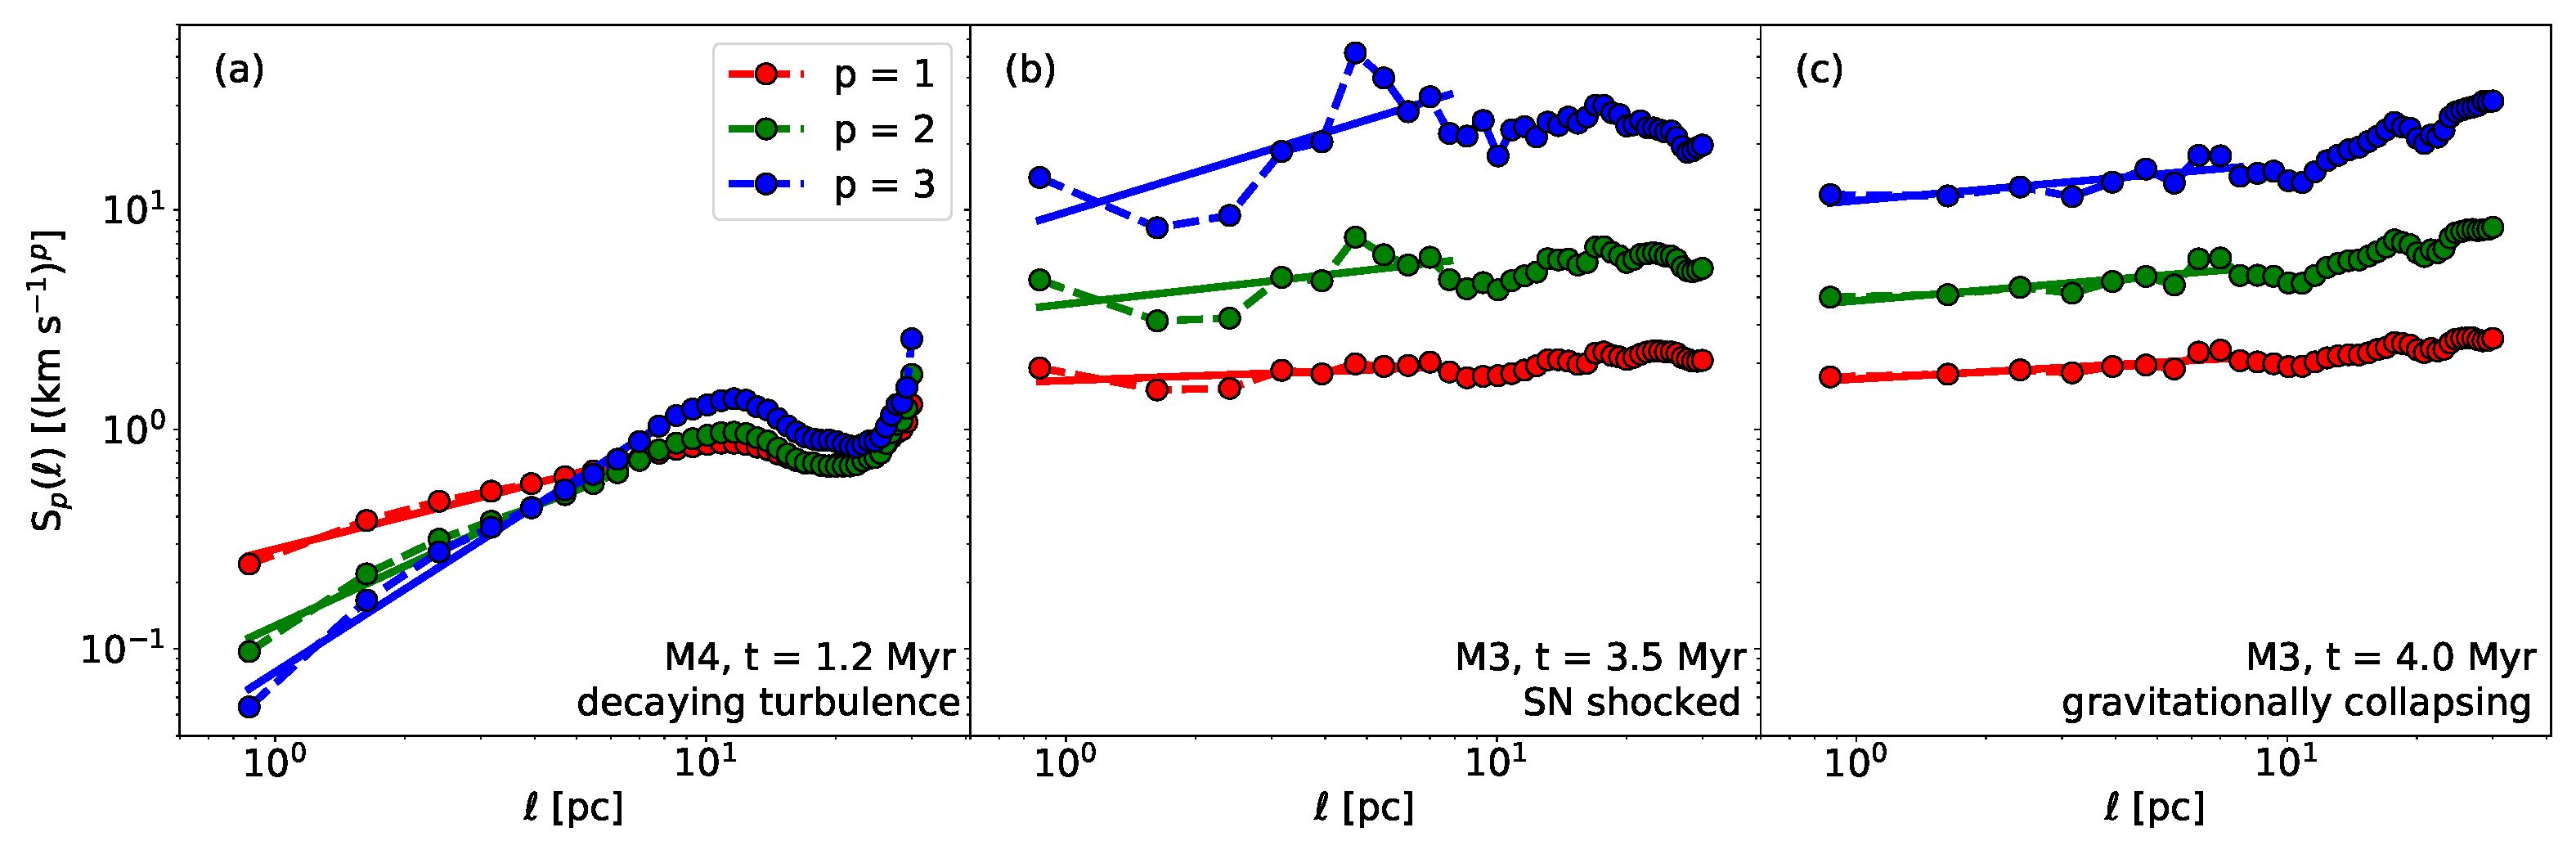
\includegraphics[width=\textwidth]{vsf_example.pdf}
	\caption{Examples of velocity structure functions as function of the lag scale $\ell$ and order $p$. 
		The dots (connected by dashed lines) show the values computed from the simulation.
		The solid lines represent the power-law relations fitted to the respective structure functions.
	}
	\label{pic:results:vsf_example}
\end{figure*}

The examples demonstrate that, in general, the measured VSFs cannot be described by a single power-law relation over the entire range of $\ell$.
Instead they are composed of roughly three different regimes: 
one at small scales at $\ell \lesssim$~3~pc, a second one within 3~pc~$\lesssim \ell \lesssim$~10--15~pc, and the last one at large scales with $\ell >$~15~pc.
\textbf{We find that} only the small and intermediate ranges may be represented by a common power-law relation.
On larger scales, one observes a local minimum before the VSFs either increase or stagnate.
Thus, in this context the VSF is an accurate tool to measure the size of a molecular cloud.
On smaller scales, which correspond to individual clumps and cores, one sees significant differences.

The examples in Fig.~\ref{pic:results:vsf_example} illustrate how VSFs react to different scenarios that affect the turbulent structure of the entire clouds. 
\textbf{Fig.~\ref{pic:results:vsf_example}(a) shows the case where turbulence is driven on large scales and naturally decays towards smaller scales.
This is the most common behavior seen in all three MCs within the first $\sim$1.5~Myr of the simulations.}
During this interval of time the clouds experience the effect of self-gravity for the first time in their evolution and need to adjust to this new condition.
Until this is the case, their VSFs are dominated by the freely cascading turbulence that previously dominated the kinetic structure of the clouds.
Furthermore, this implies that we can only reliably examine turbulence within the simulations after 1.5~Myr and carefully need to take this into account in the further discussion \citep[see][]{IbanezMejia2017,Seifried2017b}.

The other examples represent the clouds at later stages of their evolution when the VSFs are dominated by sources that drive the \textbf{flow} within the clouds in a more extreme way.
Fig.~\ref{pic:results:vsf_example}(b) shows the VSF of \texttt{M3} at a time when the cloud has just been hit by a SN shock front. 
One clearly sees how the amplitude of the VSFs is increased by one to two orders of magnitudes compared to the previous example.
Especially the power \textbf{at small scales ($\ell \lesssim$ few parsecs) is highly amplified as a result of the shock.} 
Despite the increase of turbulent power at small scales, a large amount of energy is injected at large scales, as well.
All this results in a \textbf{steeper slope of the VSF.}
However, the effect of SN shocks last for only a short period of time (see below).

The last example, Fig.~\ref{pic:results:vsf_example}(c), demonstrates the imprint of gravitational contraction.
Here, the VSF is almost flat, or even slightly increasing towards smaller separation scales. 
This kind of profile is typical for gas that is self-gravitationally contracting \citep{Boneberg2015,Burkhart2015} since gas moves into the inner regions of the cloud, reducing the average lag distances, but not necessarily the relative velocities.
The latter may even be accelerated by the infall.
As a consequence, large amounts of kinetic energy are transferred to smaller scales which flattens the corresponding VSF.

\subsection{Time Evolution}\label{results:normal}

Fig.~\ref{pic:results:zeta_all}(a) plots the time evolution of the power-law index $\zeta(p)$ fit to the \textbf{density-weighted} VSF obtained for each cloud, and each order $p$.
The figure shows several interesting features.
First, initially, at $t$~=~0~Myr, all calculated values of $\zeta$ are above the predicted values (see Eqs.~(\ref{equ:method:she}) and~(\ref{equ:method:boldyrev})).
\textbf{This suggests that we are seeing excess power at large scales from the initial convergent flows that formed the clouds.}
Second, $\zeta$ for all orders decreases with time as the clouds gravitationally collapse.
\textbf{Distributed gravitational collapse causes an increase in relative velocities at increasingly small scales as material falls into filaments and nodes.  The increase in small-scale power leads to a flattening of the VSF and thus a decrease in $\zeta$.}
Third, occasionally one observes bumps and dips in all orders of VSFs (e.g., \texttt{M3} or \texttt{M8} around $t$~=~1.7~Myr). 
These features only last for short periods of time (up to 0.6~Myr), but set in \textbf{rather abruptly and represent sudden changes in large-scale power that change the VSF slope. }

\begin{figure*}[!htb]
	\centering  
  
  \begin{subfigure}[c]{\textwidth}
      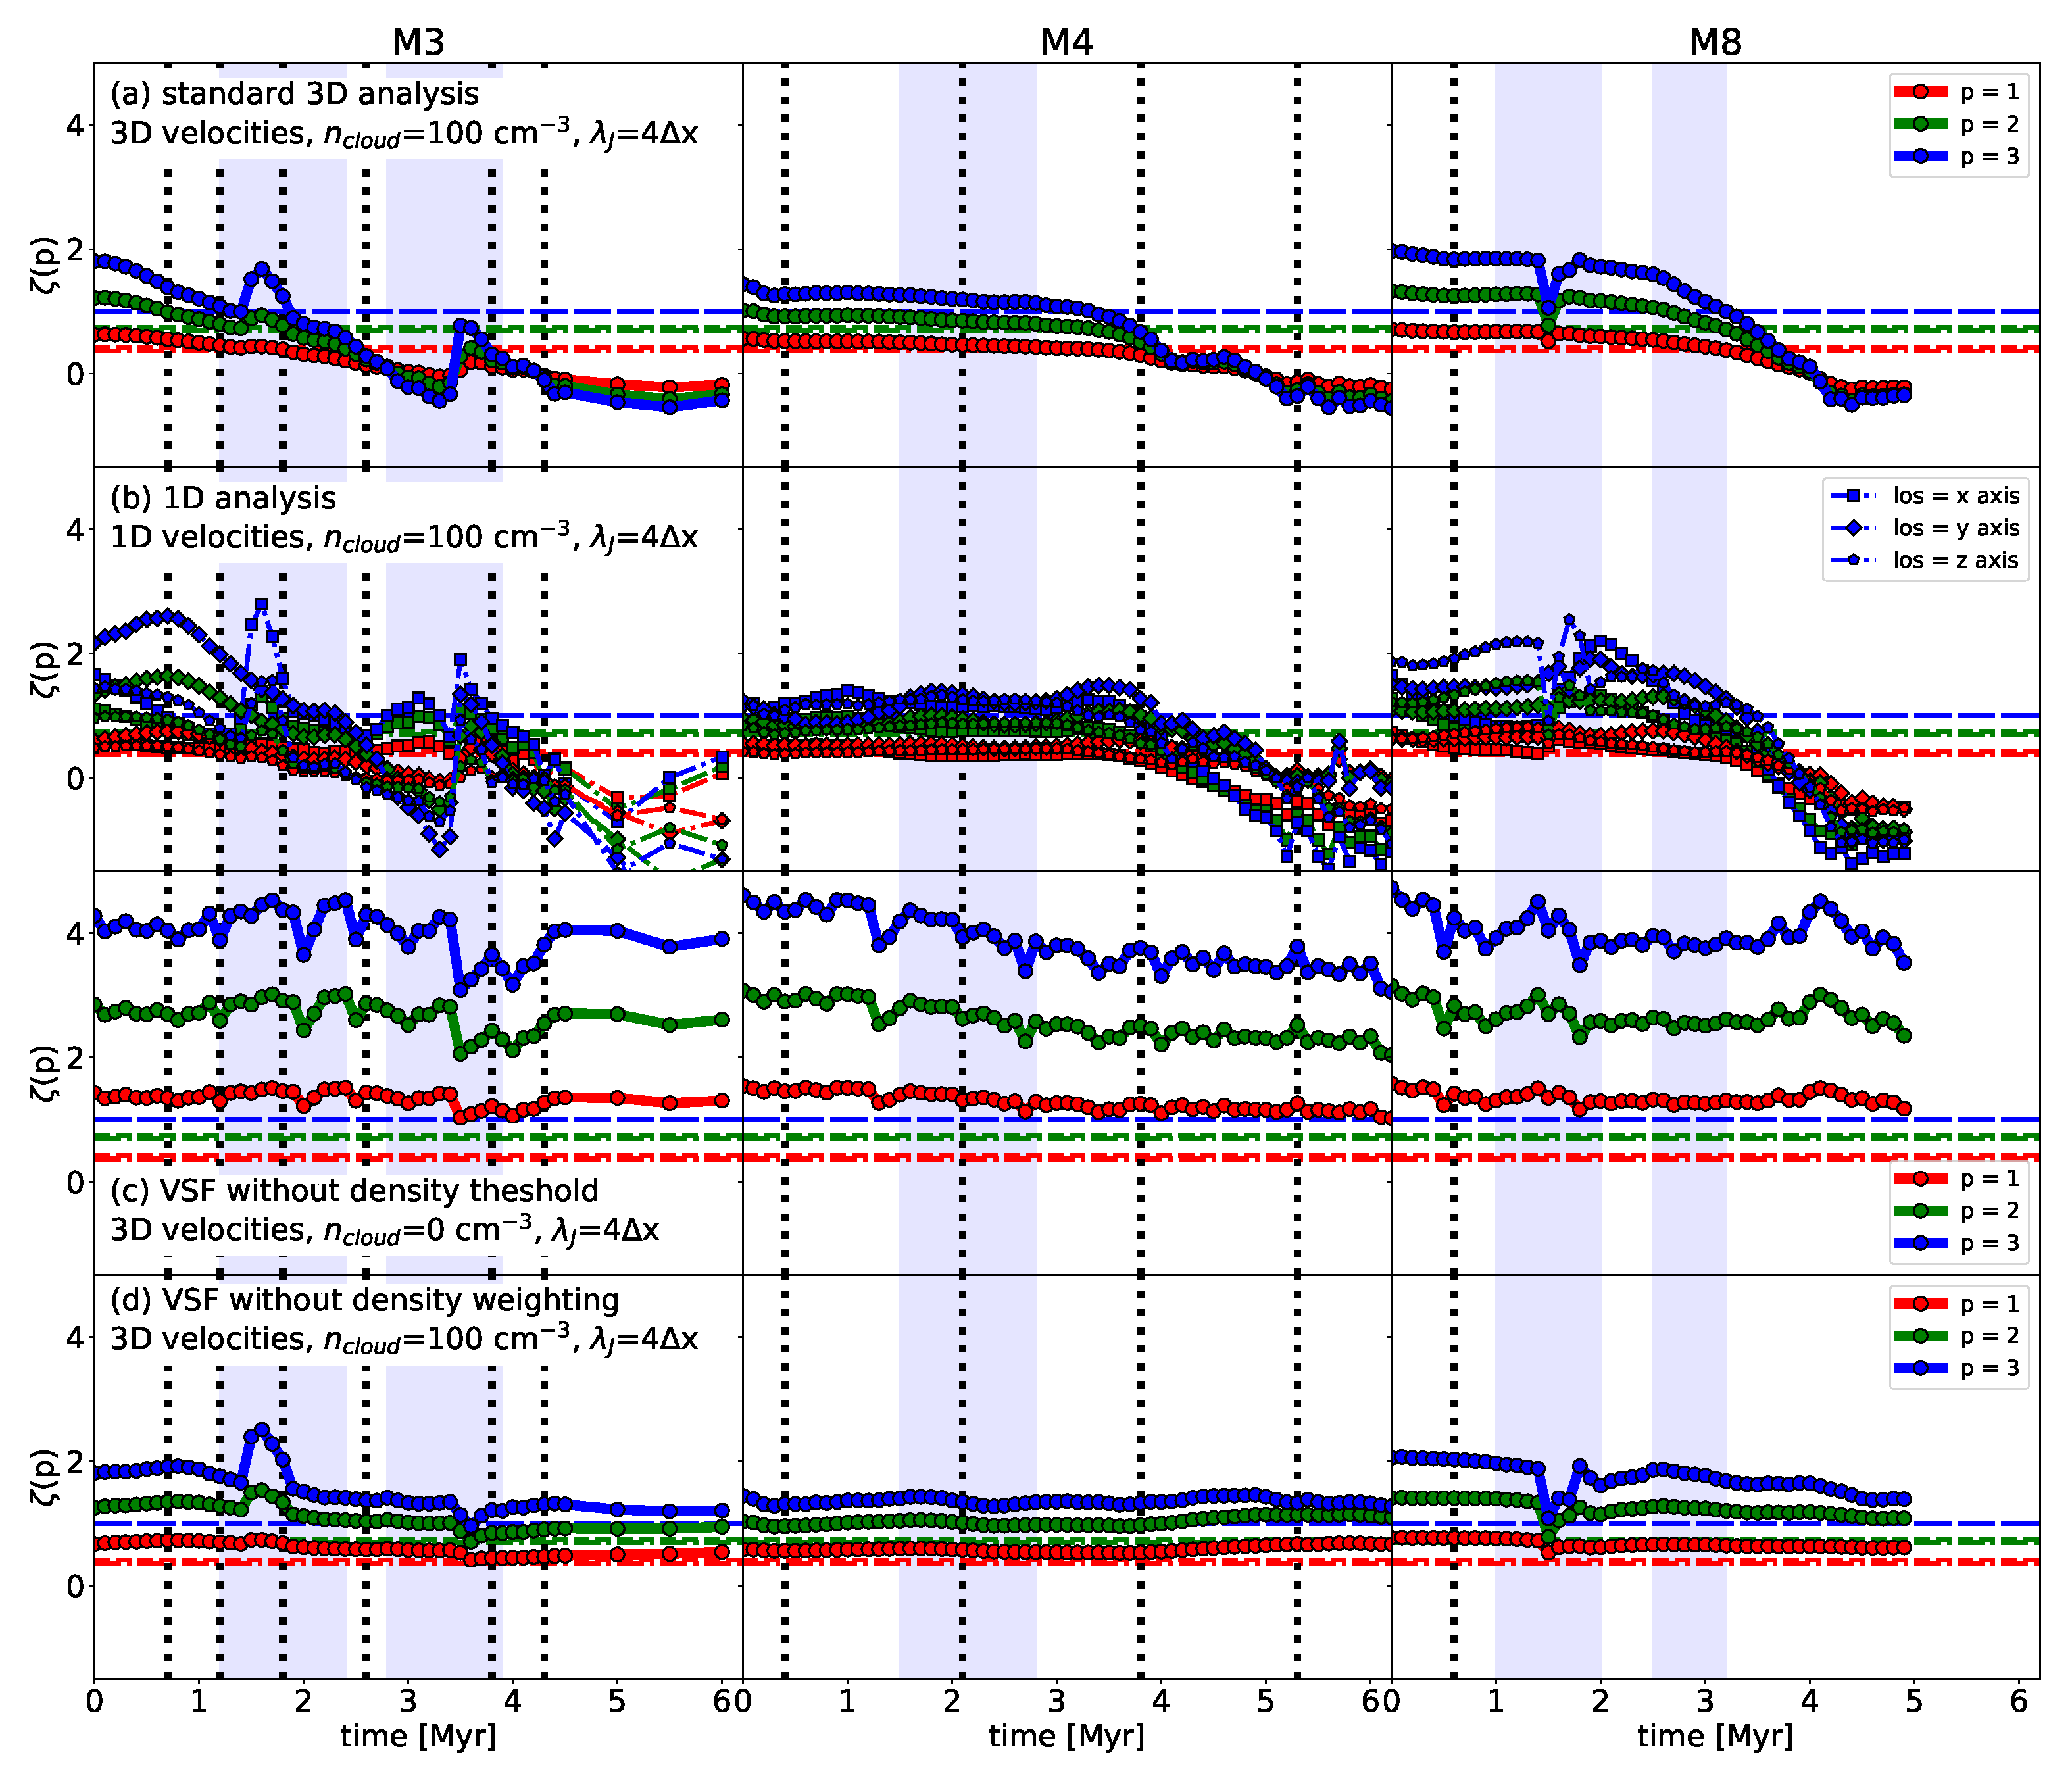
\includegraphics[width=\textwidth]{zeta_all_nojeans.pdf}
      \label{pic:results:zeta_all_nojeans}
  \end{subfigure}
  \begin{subfigure}[c]{\textwidth}
      \addtocounter{subfigure}{4}
      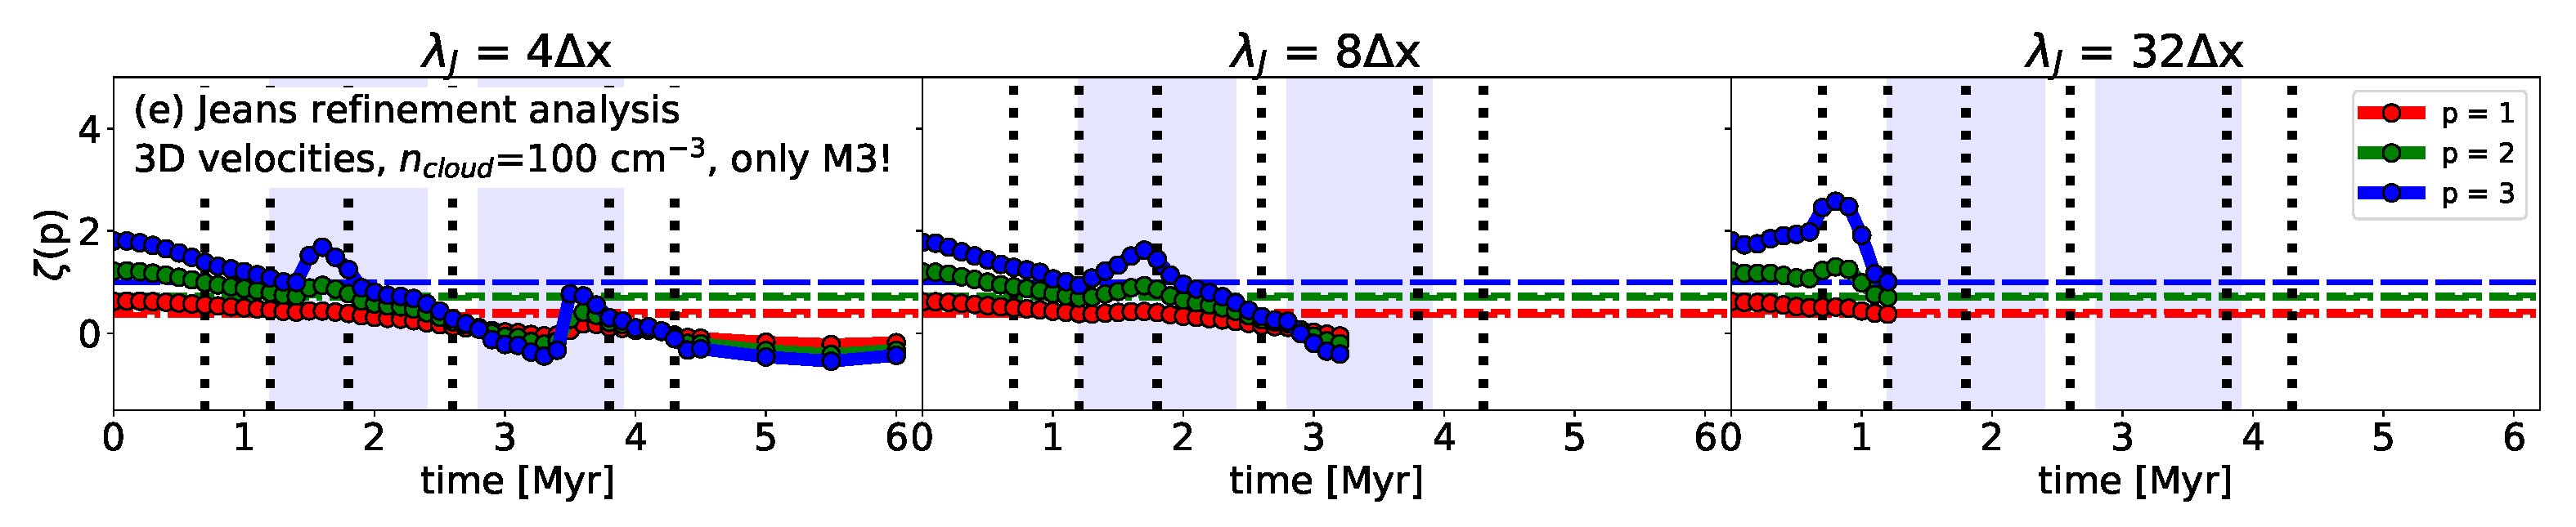
\includegraphics[width=\textwidth]{zeta_jeans.pdf}
      \label{pic:results:zeta_all_jeans}
  \end{subfigure}
  
  \caption{Time evolution of scaling exponent $\zeta(p)$ of the $p^\mathrm{th}$ order VSF. Panels (a)--(d) show the measurements for \texttt{M3}~(\textit{left}), \texttt{M4}~(\textit{middle}), and \texttt{M8}~(\textit{right}), respectively. Of these, (a) represents the standard analysis while the other rows illustrate the results of \textbf{different variations in the analysis as noted in the figures.} Panel (e) shows the values of $\zeta$ measured within \texttt{M3} as a function of the Jeans refinement level the cloud has been modelled with.  \textbf{Note that these more expensive runs were not run for as long as the fiducial run.  In all panels, the grey dotted vertical lines mark the times than a SN explodes in the vicinity of the corresponding cloud, while the blue areas indicate periods of enhanced mass accretion onto the clouds.} The coloured horizontal lines show the predicted values for \textbf{incompressible turbulence \citep[dash-dotted lines;][]{She1994} and for highly compressible, supersonic turbulence \citep[dashed lines;][]{Boldyrev2002}.}}
	\label{pic:results:zeta_all}
\end{figure*}

Fig.~\ref{pic:results:z_all}(a) shows the \textbf{corresponding} time evolution of the self-similarity parameter, $Z$. 
One sees that most of the time the measured values of $Z$ are in agreement or at least closely approaching the predicted values. 
\textbf{The occasional peaks in} $Z$ (for example, in \texttt{M4} at $t$~=~4.1~Myr) occur at times when the scaling exponents of the VSFs $\zeta(3)$ reach values close to or below 0.
The decreases in $Z$ (for example, in \texttt{M3} around $t$~=~1.8~Myr), on the other hand, occur when SN shocks hit and heavily impact the clouds, \textbf{producing stronger effects in higher order VSFs.}

\begin{figure*}[!htb]
	\centering  
  
  \begin{subfigure}[c]{\textwidth}
      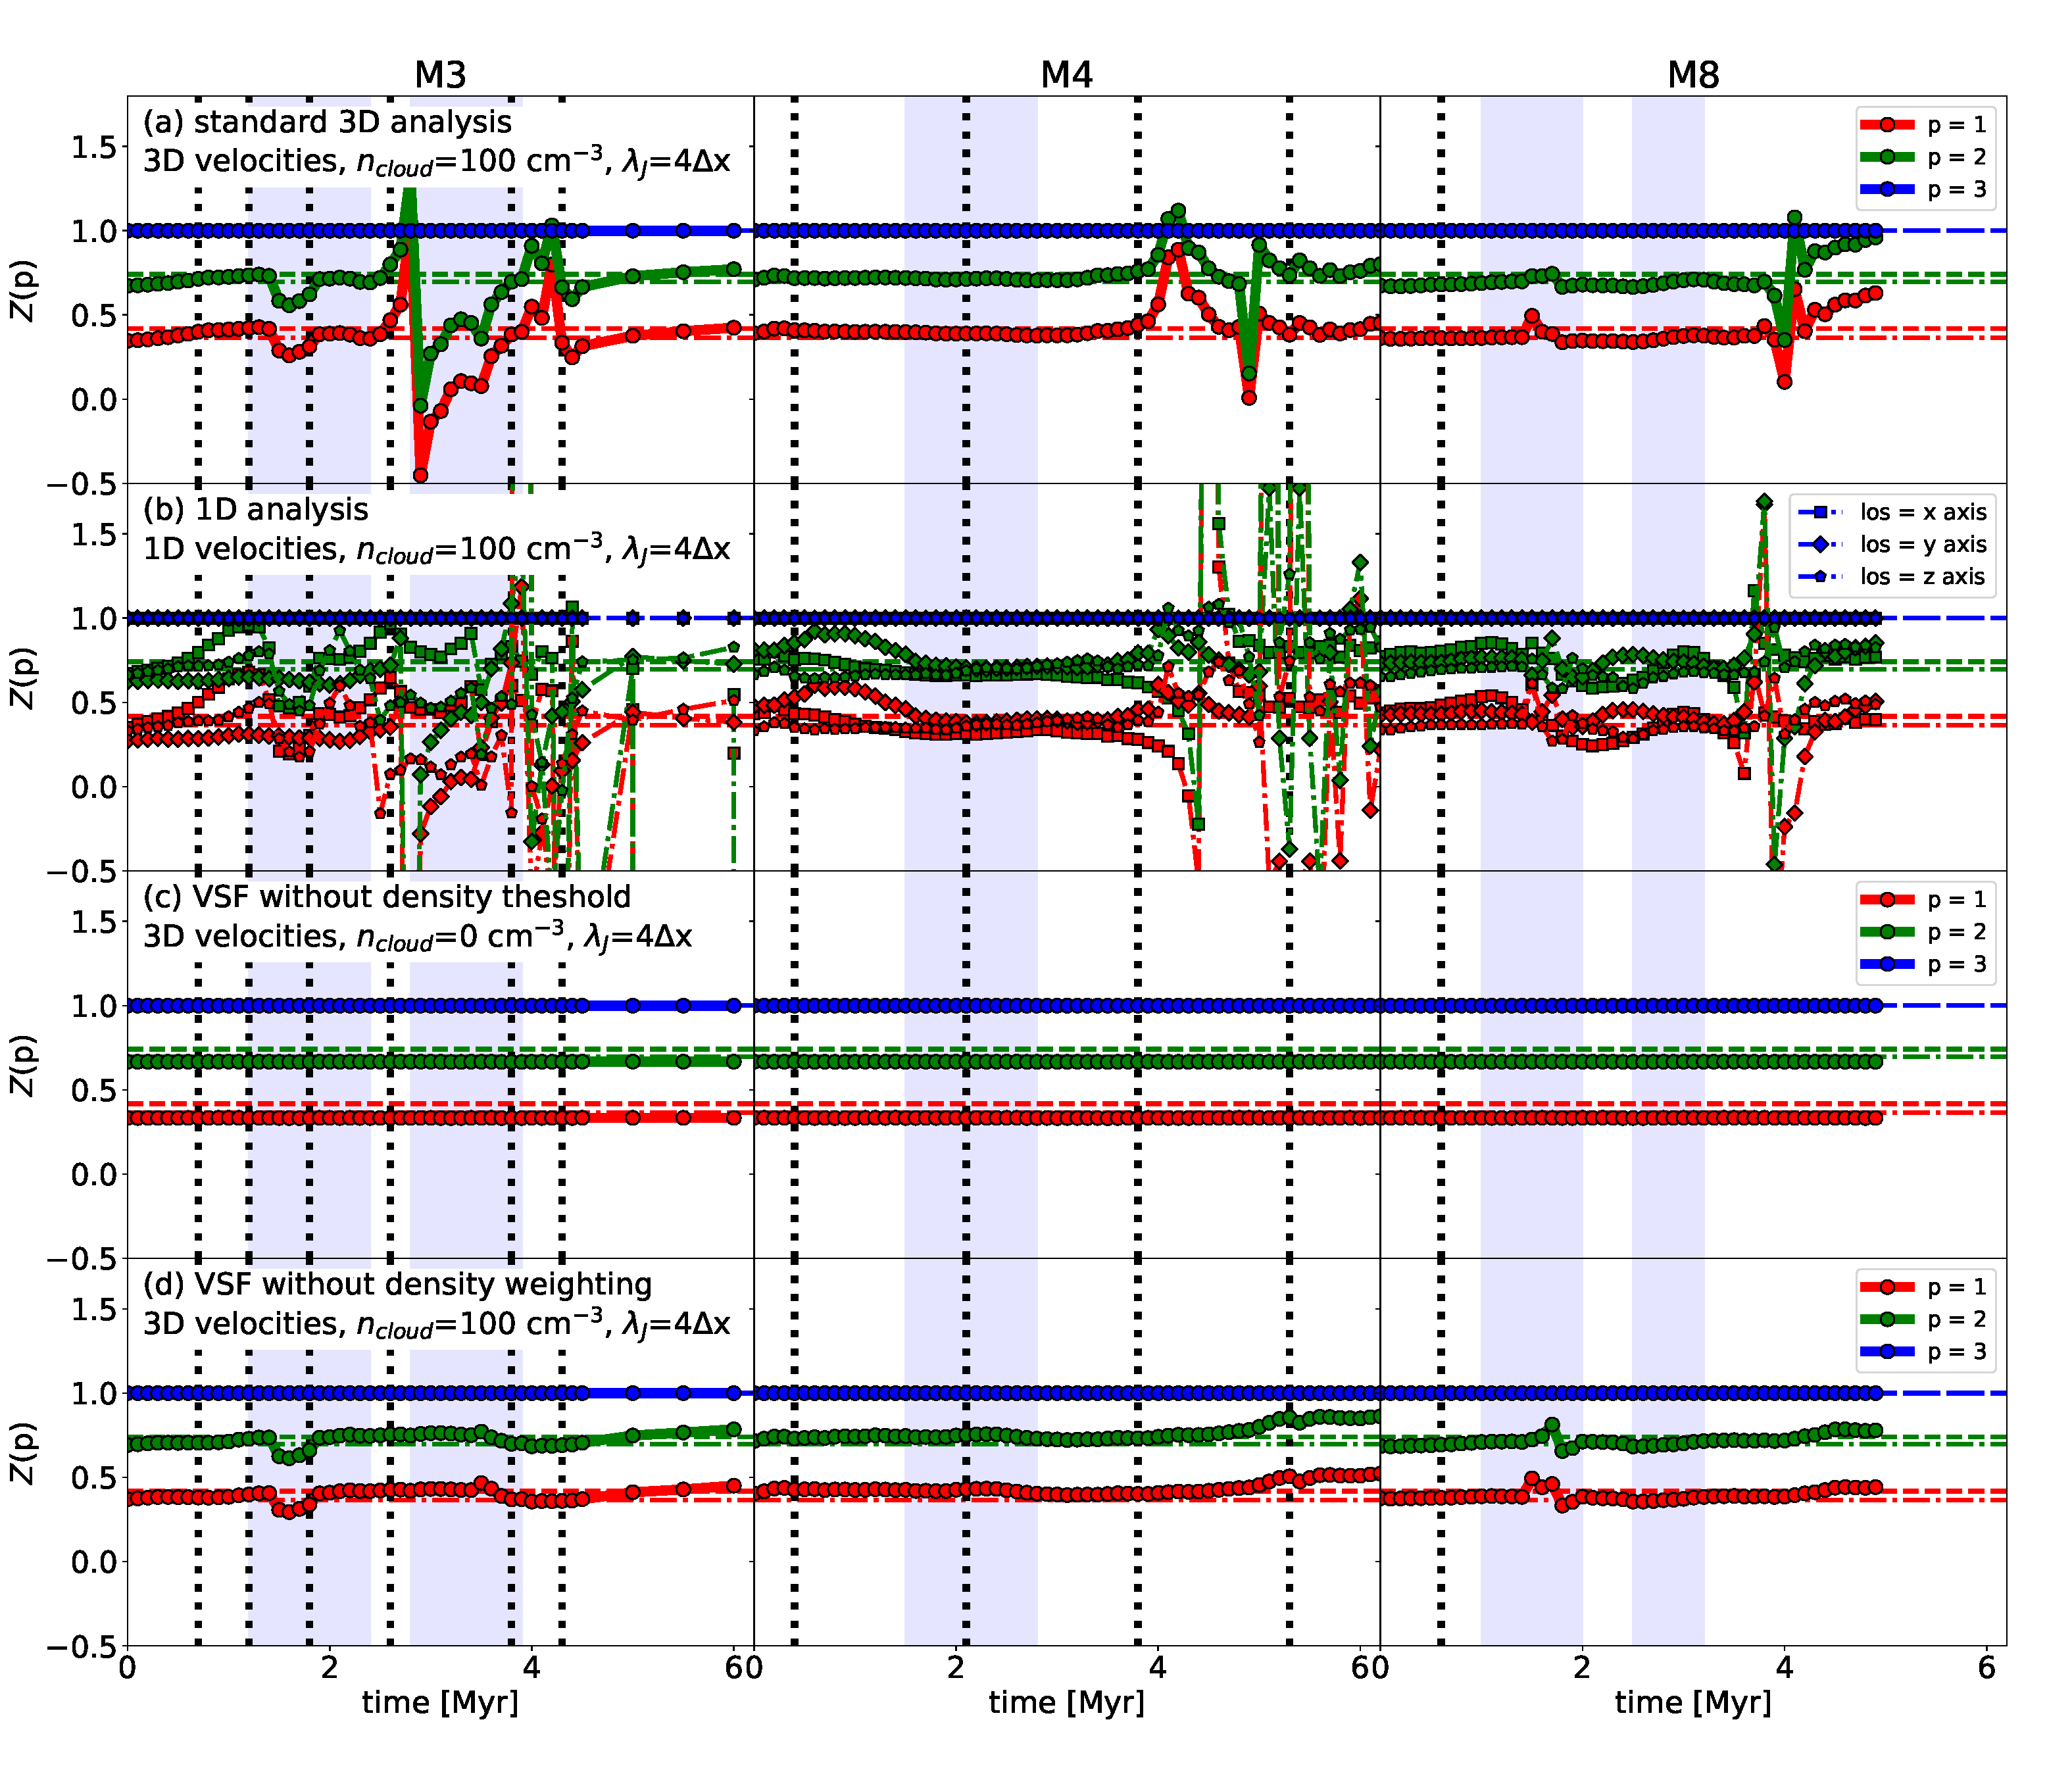
\includegraphics[width=\textwidth]{z_all_nojeans.pdf}
      \label{pic:results:z_all_nojeans}
  \end{subfigure}
  
  \begin{subfigure}[c]{\textwidth}
      \addtocounter{subfigure}{4}
      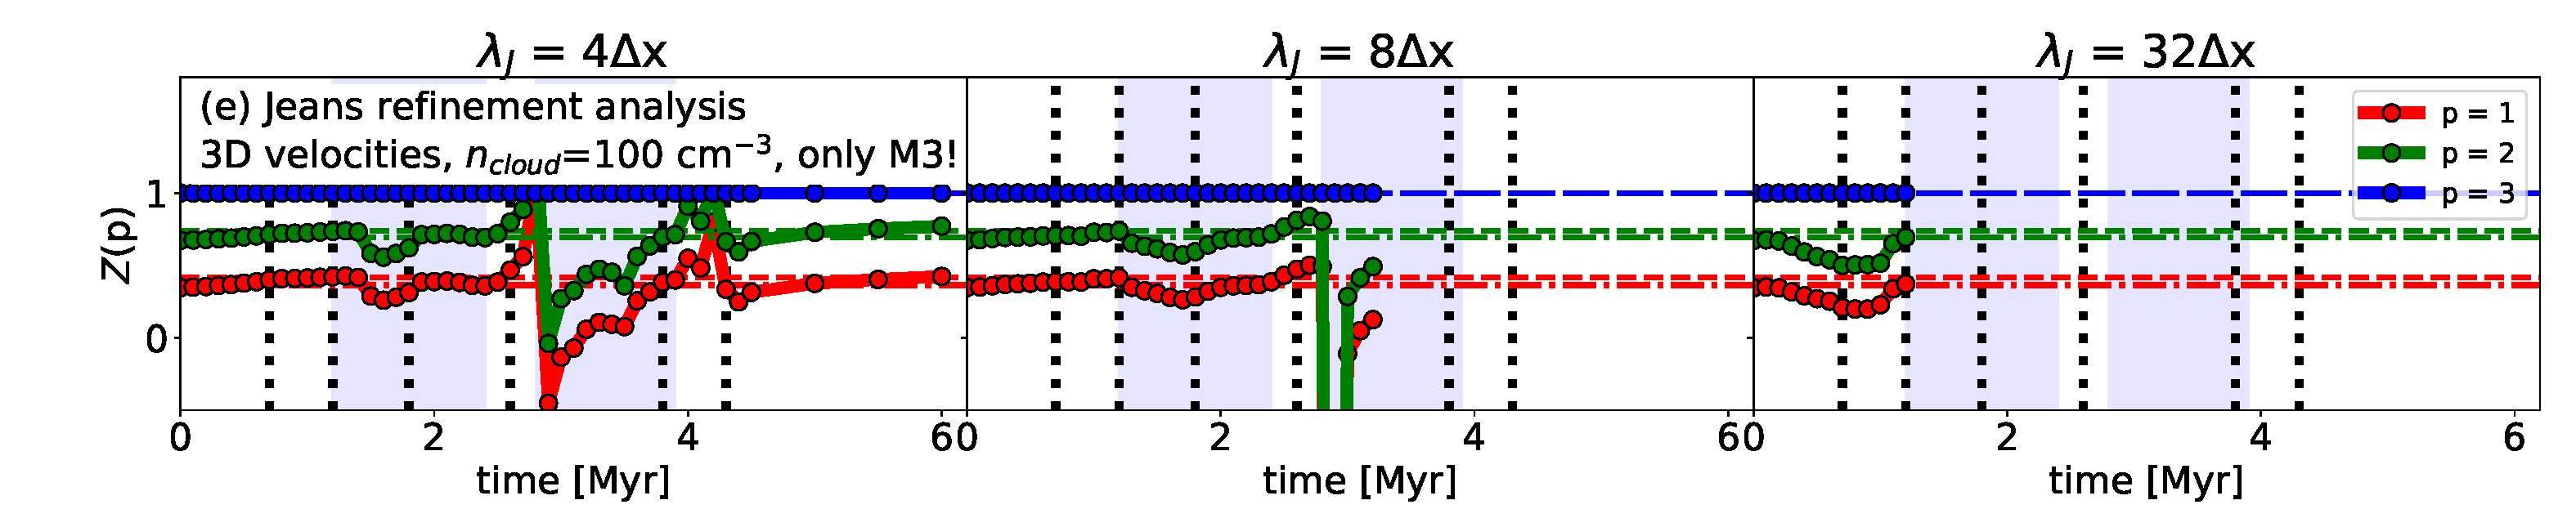
\includegraphics[width=\textwidth]{z_jeans.pdf}
      \label{pic:results:z_all_jeans}
  \end{subfigure}
  
  \caption{Like Fig.~\ref{pic:results:zeta_all}, but for the measured self-similarity parameter $Z = \zeta(p) / \zeta(3)$ of the $p^\mathrm{th}$ order VSF.}
	\label{pic:results:z_all}
\end{figure*}

In the rest of this section, we study how VSFs \textbf{computed in different ways compare to these density weighted results.}
We compare the findings with the results we have obtained with our original setup.
In Sect.~\ref{discussion}, we will discuss and interpret these results in more detail.


\subsection{Line-of-Sight VSF}\label{results:1d}

Previously, we have seen how the VSF behaves and evolves within the clouds.
By doing so, we derived the relative velocities based on the 3D velocity vectors \textbf{from the simulations.
However, observed VSFs can only be measured using line-of-sight velocities.}
Thus, in this subsection we investigate how VSFs derived from 1D relative velocities compare to the 3D VSFs presented before.

Figures~\ref{pic:results:zeta_all}(b) and~\ref{pic:results:z_all}(b) show measured $\zeta$ and $Z$, respectively, derived based on Eq.~(\ref{equ:results:def_vsf_1d}). 
We see that, in most of the cases, all 1D VSFs agree well with each other, as well as with the corresponding 3D VSFs.
Yet, there are cases in which the 1D VSF evolves temporarily or completely differently than the 3D VSF.
For example, the 1D VSF along the x-axis in \texttt{M3} initially behaves like the corresponding 3D VSF, though with lower absolute values of $\zeta$ (or higher values of $Z$).
However, during the period $t$~=~2.5--3.8~Myr the functions diverge. 
While the 3D $\zeta$ \textbf{decreases} further and switches sign, the $\zeta$ based on the 1D VSF along the $x$-axis shows a local maximum before converging with the 3D $\zeta$ again. 


\subsection{Density Thresholds}\label{results:densthres}

\textbf{We now examine the VSFs of the entire data cubes without setting a density threshold ($n_\mathrm{cloud}~=$~0~cm$^{-3}$).  Figure~\ref{pic:results:zeta_all}(c) shows $\zeta$, while Figure~\ref{pic:results:z_all}(c) shows $Z$ in this case.
These figures clearly illustrate that the measurements in the samples without density threshold completely differ from those with the density threshold.}
The measured values of $\zeta$ are much higher in the ISM than in the cloud-only sample.
Although we see a similar decline of $\zeta$ in \texttt{M4} and \texttt{M8} as the gas contracts under the influence of gravity in the vicinity of the clouds, $\zeta$ generally evolves differently here than \textbf{in the analysis that is focused on the clouds.}
We see a high rate of random fluctuations in the evolution of $\zeta$, as well.
Furthermore, contrary to all of our other test scenarios, we see here that all $Z$ are constant in time and within all clouds, with values slightly lower than those predicted by \citet{She1994} for \textbf{incompressible} flows.  
\textbf{This is consistent with the high sound speed in the hot gas that fills most of the volume of the computational box, which results in subsonic flows predominating.}


\subsection{Density Weighting}\label{results:densweight}

As mentioned in Sect.~\ref{methods:vsf}, Eq.~(\ref{equ:method:def_vsf}) represents the definition of the density-weighted VSF.
\textbf{While this represents the observational situation better, the theoretical predictions were developed for the unweighted statistic.  Thus a comparison of results for the two variations in our model is of interest. }
There are a few studies that have targeted this question 
\citep[e.g.,][]{Benzi1993,Schmidt2008, Benzi2010,Gotoh2002}.  
However, all of them considered \textbf{isotropic, homeogeneous, turbulent flows} that are not comparable to our clouds.
\citet{Padoan2016a} use both methods, but not on the same set of data. 

In this section, we investigate the influence of density weighting on VSFs by repeating the original analysis with the non-weighted VSF given by Eq.~\ref{equ:method:def_vsf}.
Figs.~\ref{pic:results:zeta_all}(d) and~\ref{pic:results:z_all}(d) show the measured values of $\zeta$ and $Z$ derived from the non-weighted VSFs, respectively.

Comparing the weighted and non-weighted samples, we see the following:
The non-weighted $\zeta$ (Fig.~\ref{pic:results:zeta_all}d) traces the interactions between the gas of the clouds and the SN shocks in the same way as occurs for the density-weighted VSF.
In \texttt{M3} and \texttt{M8} we also see that the values of $\zeta$ decrease as the clouds evolve, yet not as fast as they do in the density-weighted VSFs. 
The measurements in \texttt{M4}, however, are almost constant over time. 
In all the cases, the values of $\zeta$ never \textbf{decrease} below 0.5; a behaviour that clearly differs from what we have observed in the density-weighted VSFs. 
\textbf{The density weighting weakens the influence of the highly compressible flows in the densest regions, but not so much as in the case with no density threshold. 
Consequently, the evolution of $Z$s (see Fig.~\ref{pic:results:z_all}d) becomes smoother, as well, as there is no sign inversion of $\zeta$.
As a result the values of $Z$ fluctuate slightly when shocks hit, and otherwise vary between the compressible and incompressible limits.}



\subsection{Jeans Length Refinement}\label{results:refinement}

\textbf{The results we have discussed so far are based on simulation data presented in \citetalias{IbanezMejia2016} and \citetalias{IbanezMejia2017}.
Due to the huge computational expense of the variety of physical and numerical processes (fluid dynamics, AMR, supernovae, magnetic fields, radiative heating and cooling, and many more) within those simulations, though, they have required some compromises.
One of these compromises was the Jeans refinement criterion used as part of the AMR mechanisms.
The authors resolved local Jeans lengths by only four cells ($\lambda_J=4\Delta{}x$).
This is the minimal requirement for modelling self-gravitating gas in disks in order to avoid artificial fragmentation \citep{Truelove1998}. 
Other studies, for example by \citet{Turk2012}, have shown that a significantly higher refinement is needed to reliably resolve turbulent structures and flows within disks to resolve turbulence.  In our case, the key question is how quickly the turbulent cascade fills in after the multiple steps of refinement to higher resolution required to develop the high resolution cubes we use.  
Although we have a different physical situtation, the earlier results still emphasize the importance of how well the Jeans length is resolved.}

In the appendix of \citetalias{IbanezMejia2017}, the authors examine the effect the number of cells used for the Jeans refinement has on the measured kinetic energy.
For this, they have rerun the simulations of \texttt{M3} twice; 
once with $\lambda_J=8\Delta{}x$ for the first 3~Myr after self-gravity was activated, and once with $\lambda_J=32\Delta{}x$ for the first megayear of the cloud's evolution.
The authors show that the $\lambda_J=32\Delta{}x$ simulations smoothly \textbf{recover} the energy power spectrum on all scales already after this first megayear.
The other two setups do this, as well, \textbf{but only over longer timescales.}
This is why one can only reliably trust the findings in this paper after the clouds have evolved for approximately 1.5~Myr \citep[see also][]{IbanezMejia2017,Seifried2017b}.

Furthermore, \citetalias{IbanezMejia2017} calculated the difference in the cloud's total kinetic energy as a function of time and refinement level.
They found that the $\lambda_J = 4\Delta{}x$ simulations miss a significant amount of kinetic energy, namely up to 13\% compared to $\lambda_J = 8\Delta{}x$ and 33\% compared to $\lambda_J = 32\Delta{}x$.
However, they also observed that these differences peak around $t=0.5$~Myr and decrease afterwards, as the $\lambda_J = 4\Delta{}x$ and $\lambda_J = 8\Delta{}x$ simulations adjust to the new refinement levels.
Thus, the results we have derived from the $\lambda_J = 4\Delta{}x$ simulations need to be evaluated with respect to this lack of turbulent energy, although the clouds' dynamics remains dominated by gravitational collapse.
It also means that the $\lambda_J = 4\Delta{}x$ data become more reliable the longer the simulations evolve.

In order to study  how the level of Jeans refinement influences the behaviour of the VSFs, we investigate the \texttt{M3} data of the $\lambda_J = 8\Delta{}x$ and $\lambda_J = 32\Delta{}x$ simulations.
Figs.~\ref{pic:results:zeta_all}e and \ref{pic:results:z_all}e show $\zeta$ and $Z$ for  $\lambda_J = 8\Delta{}x$ and $\lambda_J = 32\Delta{}x$.
In Fig.~\ref{pic:results:jeans_comp} we directly compare the measurements of all refinement levels relative to $\lambda_J = 4\Delta{}x$.

$\lambda_J = 8\Delta{}x$ shows the same behaviour as $\lambda_J = 4\Delta{}x$, with values in both samples being in good agreement as the top panel of Fig.~\ref{pic:results:jeans_comp} demonstrates. 
Over the entire observed time span, the measured values of $\zeta$ decrease as the VSF become flatter.
At the time the SNe interact with the cloud, \textbf{over the course of about a megayear after traveling across the distance from the point of explosion to the cloud, the VSFs steeply increase toward larger scales causing values of $\zeta$ (Fig.~\ref{pic:results:zeta_all}e) to jump.}
Compared to the $\lambda_J = 4\Delta{}x$ sample, the peak in $\zeta$ is smoother and lasts longer \textbf{at higher Jeans resolution}.

\textbf{These same effects can be seen in Fig.~\ref{pic:results:z_all}e where the drop of $Z$ due to the SN shock lasts longer than it did for} $\lambda_J = 4\Delta{}x$. 
Besides this, the time evolution of $Z$ for $\lambda_J = 8\Delta{}x$ is as sensitive to the turbulence-related events as it was for $\lambda_J = 4\Delta{}x$.
The divergence produced when gravity has transferred the majority of power to smaller scales occurs at the same time. 
\textbf{The actual} depth of the drop is a numerical artefact caused by $\zeta(3)$ being equal or close to zero at this very time step. 

The picture changes when we analyse the VSFs based on the $\lambda_J = 32\Delta{}x$ runs (Figs.~\ref{pic:results:zeta_all}e,~\ref{pic:results:z_all}e, and~\ref{pic:results:jeans_comp}).
Here one sees that the measured values of both $\zeta$ (Fig.~\ref{pic:results:zeta_all}e) and $Z$ (Fig.~\ref{pic:results:z_all}e) are similar to those for $\lambda_J = 4\Delta{}x$ for the first 0.2~Myr.
After this short period, though, the evolution of $\zeta$ diverge. 
While $\zeta(1)$ and $\zeta(2)$ continue to decrease \textbf{similar to $\lambda_J = 4\Delta{}x$ but at lower rate,} $\zeta(3)$ increases until it peaks at $t=0.8$~Myr and falls steeply again.
This divergence has notable impact on the evolution of $Z$, as well. 
The bottom panel of Fig.~\ref{pic:results:jeans_comp} illustrates the different evolutions of measured $\zeta$ and $Z$ in the two simulations more clearly.
One sees that the differences between the samples follow the same pattern for all orders of $p$.
The differences, though, increase with the order:
While the values for $\zeta(1)$ are still in good agreement, the measured values of $\zeta(2)$ and $\zeta(3)$ for $\lambda_J = 32\Delta{}x$ are 40\% and 100\% higher than those measured for $\lambda_J = 4\Delta{}x$, respectively.
Consequently, this causes differences in $Z(p)$ of 30--52\% between the simulations.
At $t$~=~1.2~Myr, the last time step of this sample, the values of all $\zeta$ equal the measurements of $\lambda_J = 4\Delta{}x$ again.
\textbf{As the cost of extending the $\lambda_J = 32\Delta{}x$ simulation is prohibitive, we cannot determine whether this agreement will continue.}

\begin{figure*}
	\centering
    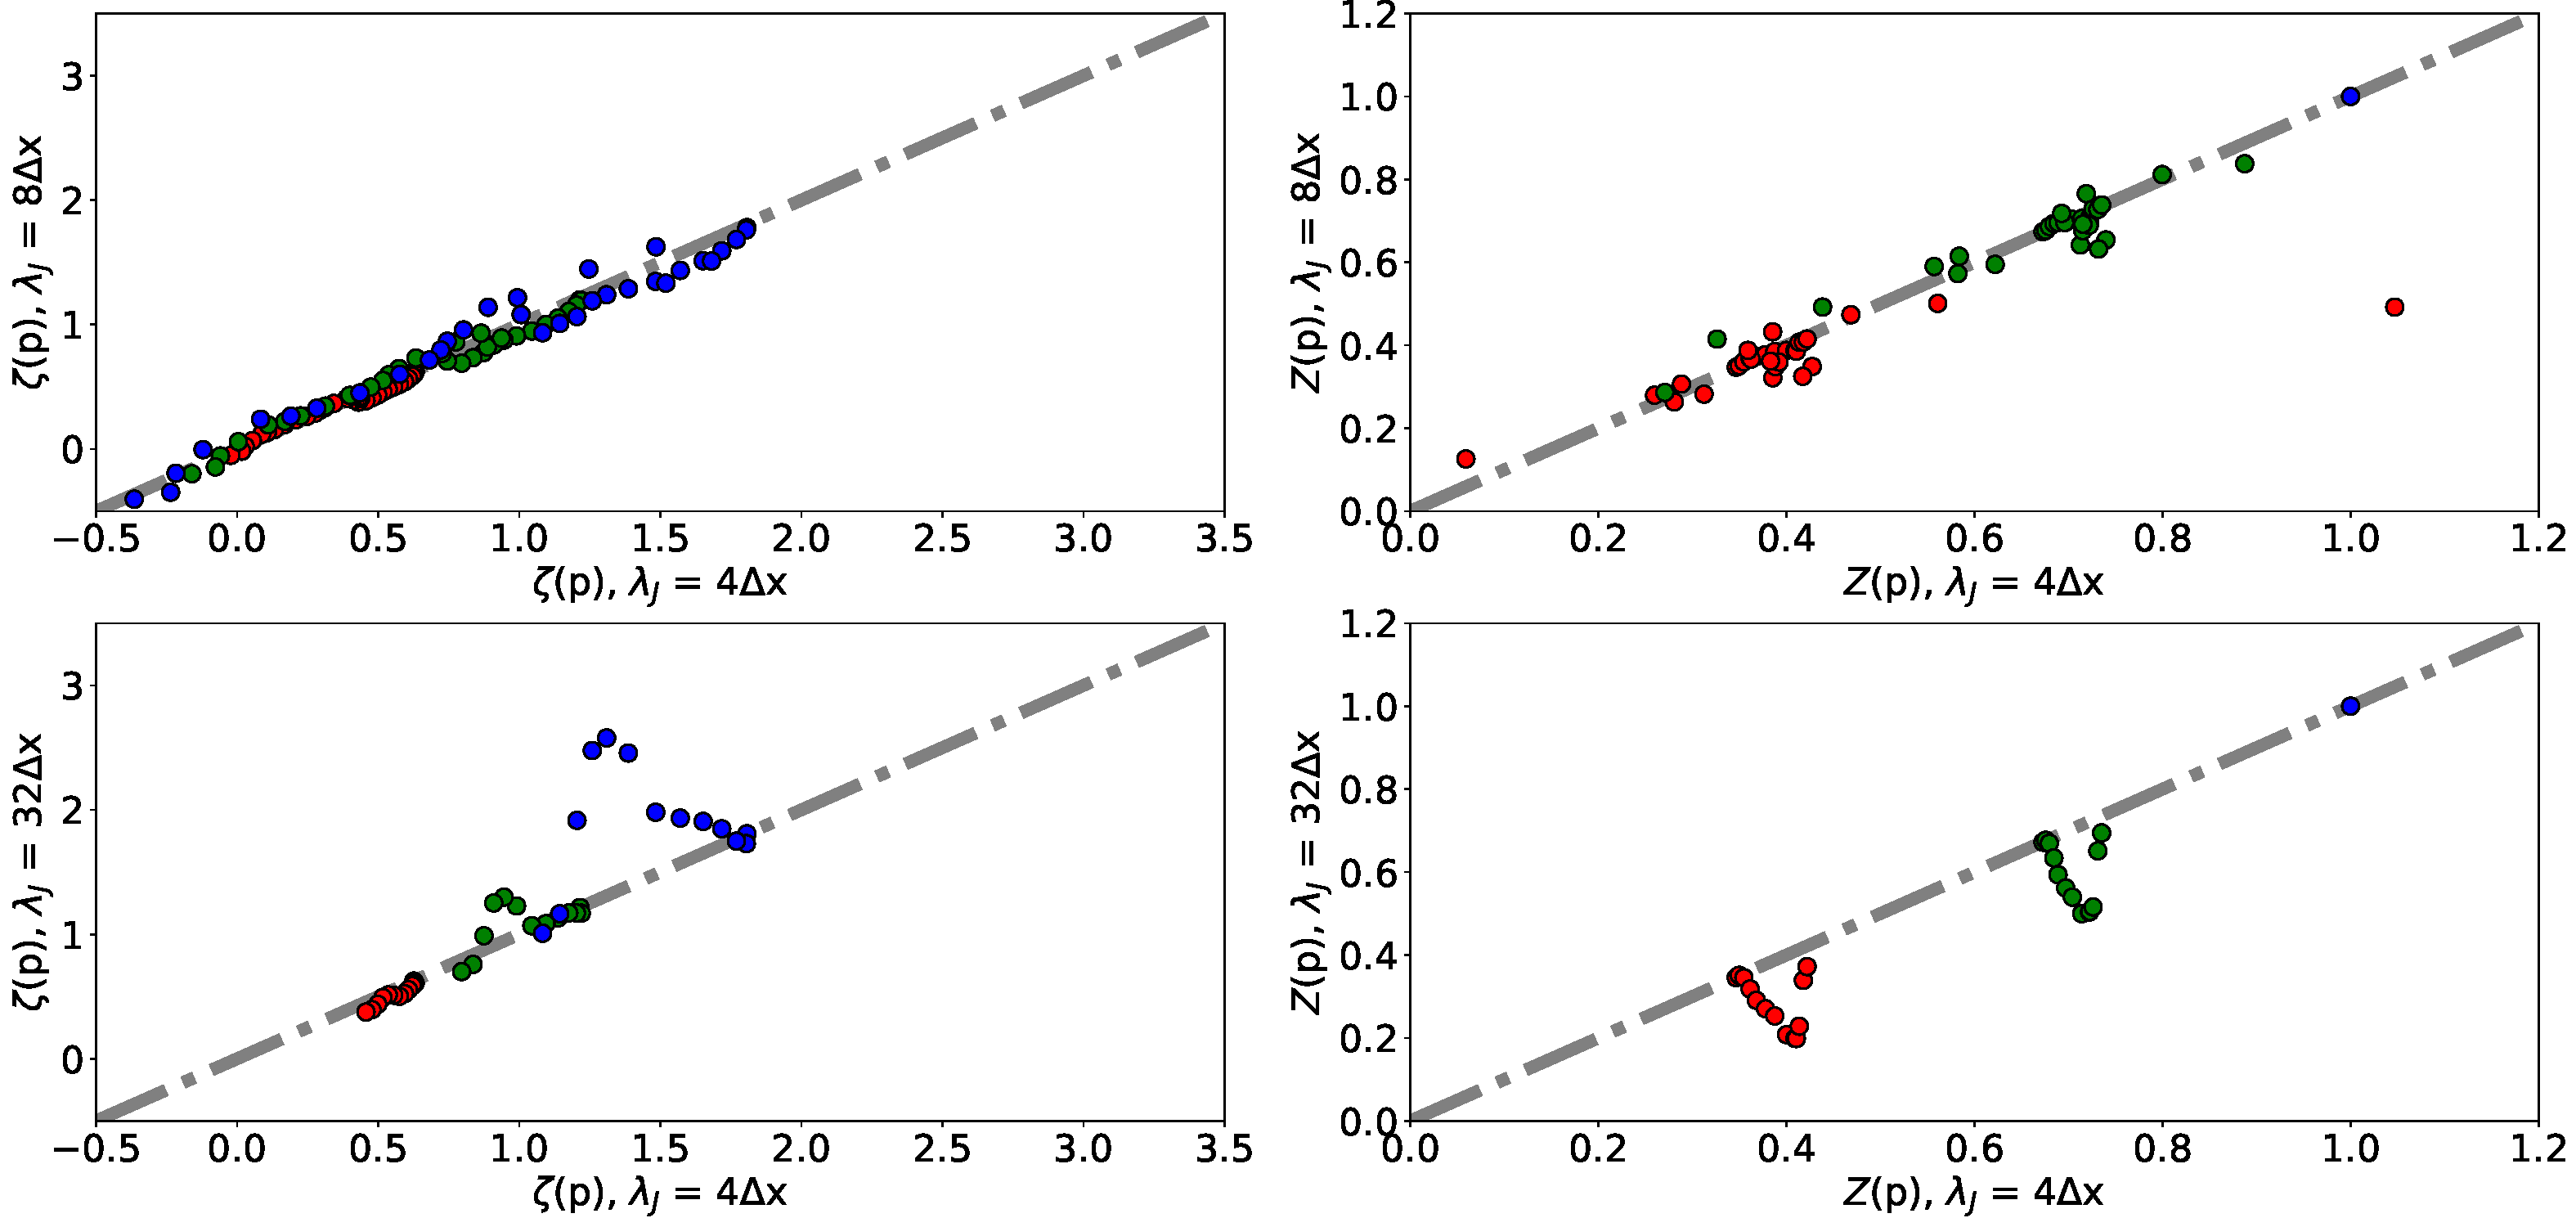
\includegraphics[width=\textwidth]{comp_jeans.pdf}
    \caption{Comparison of VSF scaling exponents, $\zeta$ (\textit{left}), and self-similarity parameters, $Z$ (\textit{right}), depending on the Jeans refinement of the simulation runs the data are based on. The abscissas give values from $\lambda_J = 4\Delta{}x$, while the ordinates give values from $\lambda_J = 8\Delta{}x$ (\textit{top}) and $\lambda_J = 32\Delta{}x$ (\textit{bottom}). All data points refer to the \texttt{M3} cloud and represent \textbf{different lags in} the same time step in the respective simulations. 
    }
    \label{pic:results:jeans_comp}
\end{figure*}


% 	\section{Discussion}\label{discussion}

\subsection{Time evolution}\label{discussion:normal}

We have seen in Sect.~\ref{results} that density-weighted VSFs reflect a combination of uniform, compressible turbulence, large-scale shocks, and gravitational collapse.  Extended self-similarity emphasises the turbulent nature of these high-Reynolds numbers flows even in regions of gravitational collapse. 

The impact of SN shocks hitting the clouds is to inject power at all scales (Fig.~\ref{pic:results:vsf_example}). 
The resulting VSFs tend to lose their power-law character. Fitting a power-law to them anyway results in substantial perturbations from the predictions for compressible turbulence even under extended self-similarity.
Fig.~\ref{pic:results:z_all} shows times of SN explosions and periods of strong accretion onto the clouds. 
Remembering that it can take the shock front more than 1~Myr to propagate from the site of the SN explosion to the molecular cloud, perturbations in $Z$ not associated with zero-crossings by $\zeta(3)$ are consistent with being caused by SN shock front interactions with the clouds.  
These shock interactions last for only a fraction of a megayear, though, consistent with the crossing time of the blast wave through the dense interior of the cloud, after which the turbulent nature of the flow reasserts itself.

As the clouds gravitationally collapse, the resulting increase in small-scale power flattens or even inverts the density-weighted VSFs, resulting in decreasing or even negative values of $\zeta$ (Fig.~\ref{pic:results:zeta_all}(a)). The increase in small-scale power can also be derived from the increasingly negative binding energy of the clouds as further gas falls into them \citepalias{IbanezMejia2017}. 
At the same time as the turbulence becomes increasingly non-uniform and anisotropic because of the importance of gravitation, the bulk velocity dispersion of the cloud increases.
\citetalias{IbanezMejia2016} showed that Eq.~(\ref{eq:larson}) is satisfied at these late times, but not at early times, less than a free-fall time, when the velocity dispersion inherited from the background turbulent flow is independent of the size of the cloud. 
These early times are when the turbulence dominates the flow and the second-order power law is roughly $\zeta(2) \simeq 1/2$.
This suggests that the apparent agreement with Larson's size-velocity relationship is coincidental, but also that observing two-point correlations using a method that cannot capture the dense flows adequately will yield this result, thus perhaps explaining the apparent success of such efforts.

Extended self-similarity shows VSF ratios characteristic of compressible turbulence (Fig.~\ref{pic:results:z_all}a), as can be seen from their tending to lie between the incompressible limit of \citet{She1994} and the extremely compressible Burgers turbulence limit of \citet{Boldyrev2002}.
(The extended self-similarity procedure fails as $\zeta(3)$ passes through zero, however, so it must be interpreted in concert with the raw values of $\zeta$.)
This suggests that, just as the extended self-similarity procedure removes the effects of dissipation, it also removes the effects of hierarchical gravitational collapse, while continuing to reflect the turbulence in these high Reynolds-numbers flows.


\subsection{Line-of-sight velocities}\label{discussion:1d}

In Sect.~\ref{results:1d} we have seen that the $\zeta$ and $Z$ derived from the 1D VSFs generally evolve similarly to those derived from the 3D VSFs.
Yet, we have also seen that individual sight lines may evolve differently.
These differences appear to reflect the detailed geometry of shock impacts on the cloud, which are reflected more strongly in the higher-order VSFs.
For example, for the first 2~Myr of the evolution of \texttt{M4} the values of $Z$ along the $y$-axis are significantly higher than those observed along the other axes and diverge significantly from the values expected for uniform turbulence.
Recall that a perturbation in $Z$ usually corresponds to an episode of strong shock driving, suggesting an impact along the $y$-axis at this time. 
Along the other two axes, $Z$ continues to agree with supersonic turbulence \citep{Boldyrev2002}.
This effect is only visible as we analyse the three dimensions separately, while the driving of the gas along the $y$-axis is averaged out in the 3D VSFs (see Fig.~\ref{pic:results:z_all}a).

In summary, for a fully developed 3D turbulent field we expect that 1D VSFs behave similarly to 3D VSFs.
However, when there is a preferred direction along which the gas flows, the 1D and 3D VSFs differ significantly from each other. 
Thus, we predict that observed VSFs reflect the nature of turbulence within MCs unless there is clear evidence that the gas is driven in a particular direction (e.g., by a stellar wind or SN shock front).

Note that this analysis does not take typical line-of-sight effects, such as optical depth or blending, into account. 
Future studies need to investigate this point in more detail by performing VSF analyses based on full radiative transfer calculations.



\subsection{Density thresholds}\label{discussion:densthres}

We find that the structure and behaviour of VSFs strongly depends on whether or not we assume a density threshold in computing them.
In the fiducial case, where n$_\mathrm{cloud}$~=~100~cm$^{-3}$, we have seen a mostly straight decline of $\zeta$ while $Z$ remains fairly constant over time, reflecting the contraction of the clouds due to self-gravity.
On the other hand, if we remove the density threshold, including the entire high-resolution cube in the calculation, we observe a completely different picture.
The high velocities present in the diffuse interstellar medium surrounding the cloud lead to strong large-scale power and thus much steeper VSFs, corresponding to higher values of $\zeta$. 
There is still a slightly declining trend in $\zeta$, but the evolution is dominated by random fluctuations.
We also see that $Z$ remains constant for the entire simulation in every case.
The VSFs for the entire box appear consistent with the prediction for the value in incompressible turbulence \citep{Boldyrev2002}. 
This suggests that they are dominated by the subsonic flow in the hot gas with $T > 10^6$~K that occupies most of the volume of the box.

Furthermore, the results demonstrate that the effect of SNe, and the interaction of the produced shock fronts with the ISM acts rather locally. 
This means that a single SN can not drive the gas dynamics on scales of our entire cubes (40$^3$~pc$^3$), at least not in the same way as it does on scales of individual MCs.
Rather the VSFs reflect the superposition of multiple SNe that only combined drive the turbulence of the diffuse ISM.

We conclude that the decision of whether or not a density threshold is used has a significant and direct influence on the resulting VSFs.
Indeed, it is a straight-forward approach to focus the analysis on the actual area of interest.
In observational studies such a threshold will anyway always be present as minimal collision rates for excitation or the sensitivity of detectors automatically introduce implicit density or intensity thresholds. 
Although we have only tested two specific setups in this context we have seen the significance of a proper choice of the density threshold, as well as a proper discussion of the obtained results considering the threshold as one of the defining parameters.




\subsection{Density weighting}\label{discussion:densweight}

In this subsection, we discuss the effect of computing the VSF with or without including density weighting, relying on the results presented in Sect.~\ref{results:densweight}.
As long as the turbulence is dominated by the large scales, and a density threshold is used, considering the density weighting does not have a significant effect.
However, as the clouds evolve the differences increase:
the non-weighted VSFs never drop below 0.5.
This is because the non-weighted VSF treats all cells equally, no matter whether the particular cell represents a dense element of the cloud centre or a diffuse element of the cloud's edge, while the weighted VSF gives more weight to the matter within the small-scale, dense, collapsing regions.
The kinetic energy is dominated by these regions.
Thus, neglecting density weighting decouples the VSF from the kinetic energy distribution.
(A more exact treatment of this question is given by \citet{Kritsuk2013a} and \citet{Banerjee2017,Banerjee2018}.)
This is particularly important at late times when small-scale collapse dominates.

Nevertheless, Fig.~\ref{pic:results:z_all}(d) illustrates that these differences do not prevent extended self-similarity from holding. 
Regardless of whether density-weighting is included, the values of $Z$ remain similar, with similar responses to external driving, except for the features created when $\zeta(3)$ passes through zero in the density-weighted VSFs.
This observation is true for all Jeans refinement levels, as Fig.~\ref{pic:results:comp_weighting} demonstrates.


\begin{figure*}
	\centering
    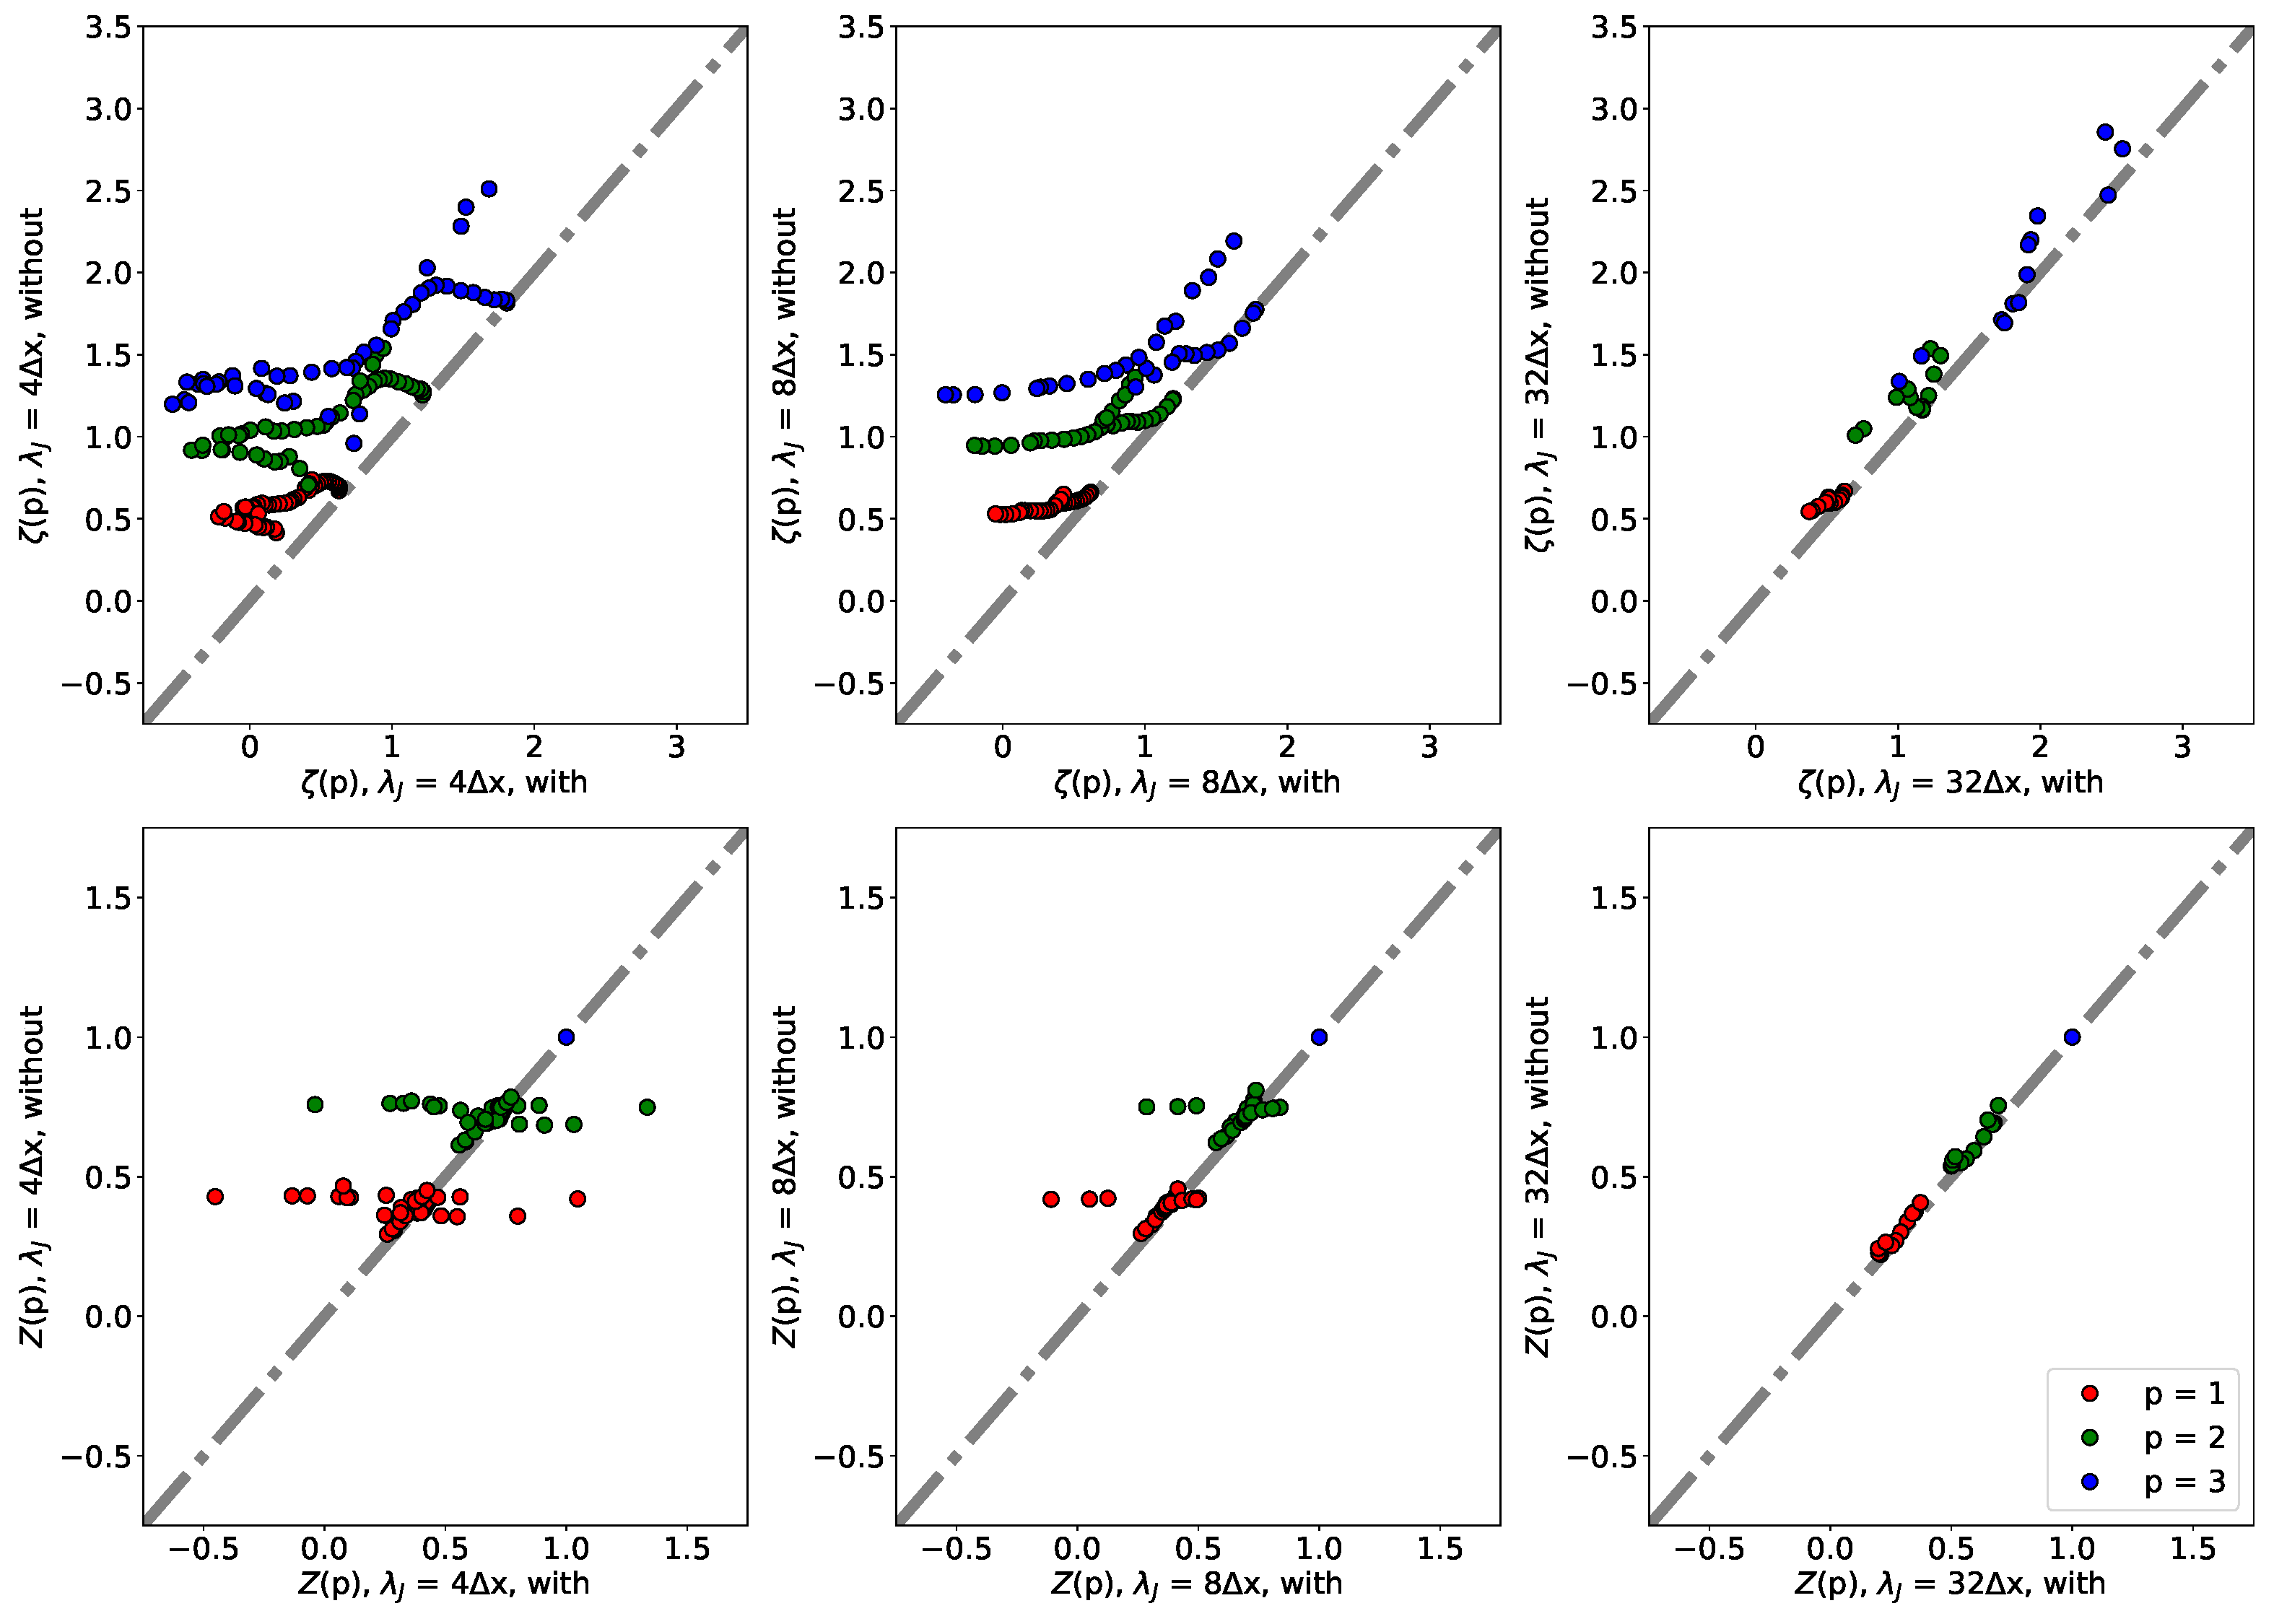
\includegraphics[width=\textwidth]{comp_weighting.pdf}
    \caption{ Comparison of $\zeta$ (\textit{top}) and $Z$ (\textit{bottom}) measured based on density-weighted VSFs (\textit{abscissas}) and non-weighted VSFs (\textit{ordinates}). We note that the given values are based on \texttt{M3} only.}
    \label{pic:results:comp_weighting}
\end{figure*}

Fig.~\ref{pic:results:comp_weighting} summarises the comparison of $\zeta$ and $Z$ measured with the density-weighted and non-weighted VSFs for all Jeans refinement levels (meaning the granularity used for modelling the turbulent motions of the gas, see Sect.~\ref{results:refinement} for more details).
The figure clearly shows that the measurements only agree well for the highest refinement level with $\lambda~=~32\Delta x$.
However, we would need more data points to be sure that this correlation is indeed real.
At lower refinement levels the measurements, as those used for the standard analysis and all other test scenarios but the one presented in Sect.~\ref{results:refinement}, correlate less well with each other. 
The differences in the samples appear dominantly when the density-weighted $\zeta$ cease below $\approx$0.5, which is the global minimum for the non-weighted $\zeta$. 
This means that none of the $\zeta$ computed in all clouds and refinement levels with the non-weighted VSF is measured to be below 0.5.

We conclude that deriving the VSF from smooth density distributions without considering density-weighting does not affect the behaviour of $\zeta$ and $Z$, as long as the turbulence is dominated by large scale flows, but it has a significant effect on the measurements when the small scales become dominant.
The latter is particularly important as this finding has a directly impact on the conclusions drawn based on the scales and mechanisms that drive the turbulence based on the measured $\zeta$.
Not only does $\zeta$ become insensitive to the influence of gravitational contraction with time, the non-weighted VSFs also does not reflect when the majority of kinetic energy has been transferred to small scales. 
Furthermore, this emphasises the importance of taking optical depth effects into account, as single tracers covering limited density ranges may effectively provide statistics closer to the non-weighted VSFs.



\subsection{Jeans length refinement}\label{discussion:refinement}

In Fig.~\ref{pic:results:jeans_comp} we see that the choice of refinement level has no significant influence on the measurements and evolution of both $\zeta$ and $Z$. 
The $\lambda_J=4\Delta{}x$ and $\lambda_J=8\Delta{}x$ models are in good agreement with each other.
This means that, although refining Jeans lengths with 4~cells misses about 13\% of kinetic energy, the effect on the structure and behaviour of the turbulence is rather small and not traced by the VSF analysis.

However, Fig.~\ref{pic:results:jeans_comp} shows that the agreement is rather poorer with $\lambda_J=32\Delta{}x$, as the latter differs more from $\lambda_J=4\Delta{}x$ the higher the order of the VSF is.
Following the explanations in Sect.~\ref{results:refinement}, the behaviour of $\zeta$ and $Z$ in the $\lambda_J=32\Delta{}x$ runs corresponds to the reaction of the cloud's gas to a shock wave running through the cloud; caused by a SN that exploded before $t$~=~0~Myr. 
Indeed one sees a SN at a distance of 172~pc at $t=-1.11$~Myr. 
As the power of the shock decreases rapidly with distance, the SN is too weak to effectively compress the gas within \texttt{M3}.
This is why it was not detected in the less refined samples.

The SN explodes far below the mid-plane of the simulated disk galaxy, in a region without dense gas, so the blast wave remains strong as it propagates through the ISM. 
By the time the blast arrives at cloud \texttt{M3}, it is still energetic enough to impact the cloud with winds at velocities above 300~km~s$^{-1}$, at the closer edge of the cloud. 
This causes an increase of VSFs at longer lag scales and the increase of $\zeta$, as well as the drop in $Z$.
However, in the less refined runs the arrival of the blast wave only contributes to the normal external driving for the gas' turbulence.
Only the $\lambda_J=32\Delta{}x$ runs can capture the fine structure of the shock driven into the cloud by the blast wave, which is why we detect this feature in these runs only. 
This emphasises the importance for studies like ours of properly resolving the full internal structure of realistic MCs.

We conclude that improving the resolution resolves details that can affect the VSF, but that the overall behaviour is already determined by our moderate resolution simulations.

\subsection{Comparison to observations}\label{discussion:observation}

The majority of studies of VSFs in MCs are based on simulated data, as is the work presented in this paper.
However, there are also some surveys that derive VSFs from observations, or whose data can be used to reconstruct the scaling properties of VSFs. 
In this section we discuss our results in the context of the observational studies that we list in Table~\ref{tab:discussion:summary_obs}.

%mm [removed use of multirow and excess lines to stay within standard A&A style]
\begin{table*} 
\centering 
	\begin{tabular}
%mm {l|l|ccc}
        {llccc} 
	\centering 
		Reference & Comments & p & $\zeta$ & Z \\ \hline  \hline
		
%mm \multirow{2}{*}{ }
\citet{Heyer2004} & $^{12}$CO J = 1-0, & 
               %mm \multirow{2}{*}{
                   1 &  
              %mm \multirow{2}{*}{
                     0.49 $\pm$  0.15 &  
                             %mm \multirow{2}{*}{
                                          0.49 $\pm$  0.15 \\ 
					& Perseus \& Solar Neighborhood & & & \\ \hline
%mm \multirow{2}{*}{
             \citet{Heyer2015} & $^{12}$CO \& $^{13}$CO J = 1-0, 30 MCs & 1 &  0.24 $\pm$  0.00 &  0.24 $\pm$  0.00 \\ 
					 & $^{12}$CO \& $^{13}$CO J = 1-0, Taurus & 1 &  0.26 $\pm$  0.00 &  0.26 $\pm$  0.00 \\  \hline
%mm \multirow{2}{*}{
           \citet{Miesch1994} & $^{13}$CO J = 1-0, & 1 &  0.43 $\pm$  0.15 &  0.43 $\pm$  0.15 \\ 
					   & 12 clouds and subregions of GMCs & 2 &  0.86 $\pm$  0.30 &  0.86 $\pm$  0.30 \\  \hline
%mm \multirow{6}{*}{
     \citet{Padoan2003} & 
     %mm \multirow{3}{*}{
         $^{13}$CO J = 1-0, Perseus & 1 &  0.50 $\pm$  0.00 &  0.42 $\pm$  0.00 \\ 
					   &  & 2 &  0.83 $\pm$  0.00 &  0.72 $\pm$  0.00 \\ 
					   &		 & 3 &  1.18 $\pm$  0.00 &  1.00 $\pm$  0.00 \\ 
					  & 
       %mm \multirow{3}{*}{
              $^{13}$CO J = 1-0, Taurus & 1 &  0.46 $\pm$  0.00 &  0.42 $\pm$  0.00 \\ 
					   &		 & 2 &  0.77 $\pm$  0.00 &  0.72 $\pm$  0.00 \\ 
					   &		 & 3 &  1.10 $\pm$  0.00 &  1.00 $\pm$  0.00 \\  \hline
		\citet{Padoan2006} & $^{13}$CO J = 1-0, Perseus & 2 &  0.80 $\pm$  0.10 &  0.80 $\pm$  0.10 \\  \hline
		\citet{RomanDuval2011} & $^{13}$CO J = 1-0, 367 clouds from the GRS survey & 1 &  0.50 $\pm$  0.30 &  0.50 $\pm$  0.30 \\  \hline
%mm \multirow{4}{*}{
\citet{Zernickel2015} & 
         %mm \multirow{2}{*}{
                   $^{13}$CO J = 1-0, NGC 6334 & 1 &  0.38 $\pm$  0.00 &  0.38 $\pm$  0.00 \\ 
					   &		 & 2 &  0.76 $\pm$  0.01 &  0.76 $\pm$  0.01 \\ 
					 & 
                 %mm \multirow{2}{*}{
                      $^{13}$CO J = 1-0, NGC 6334, $\ell \leq$ 4 pc  & 1 &  0.48 $\pm$  0.01 &  0.48 $\pm$  0.01 \\ 
					   & & 2 &  0.79 $\pm$  0.01 &  0.79 $\pm$  0.01 
	\end{tabular} 
	\caption{Summary of observed $\zeta$ and Z in the literature.} 
	\label{tab:discussion:summary_obs} 
\end{table*} 


Most of the velocity information derives from $^{12}$CO and $^{13}$CO observations of young star-forming regions \citep[e.g., Perseus and Taurus][]{Padoan2003}.
We also consider observations of more evolved regions, such as those of the H~{\sc ii} region NGC 6334 \citep{Zernickel2015}, since the filaments in our simulated MCs fragment within the first 2 Myr \citepalias{Chira2018}, suggesting that our cloud may start to resemble such more evolved regions.

Fig.~\ref{pic:discussion:comp_observation} summarises the measured scaling exponents found in the literature, along with our fiducial results (Figs.~\ref{pic:results:zeta_all}a).
We see that the observed values of $\zeta$ are in general close to each other, as well as to the predicted values by \citet{She1994} and \citet{Boldyrev2002}. 
Furthermore, we see that the observed values are always positive, suggesting that none of the observed clouds show signs of being dominated by collapse, though that could be because the fastest flows lie in optically thick regions inaccessible to the observations.  

\begin{figure}
	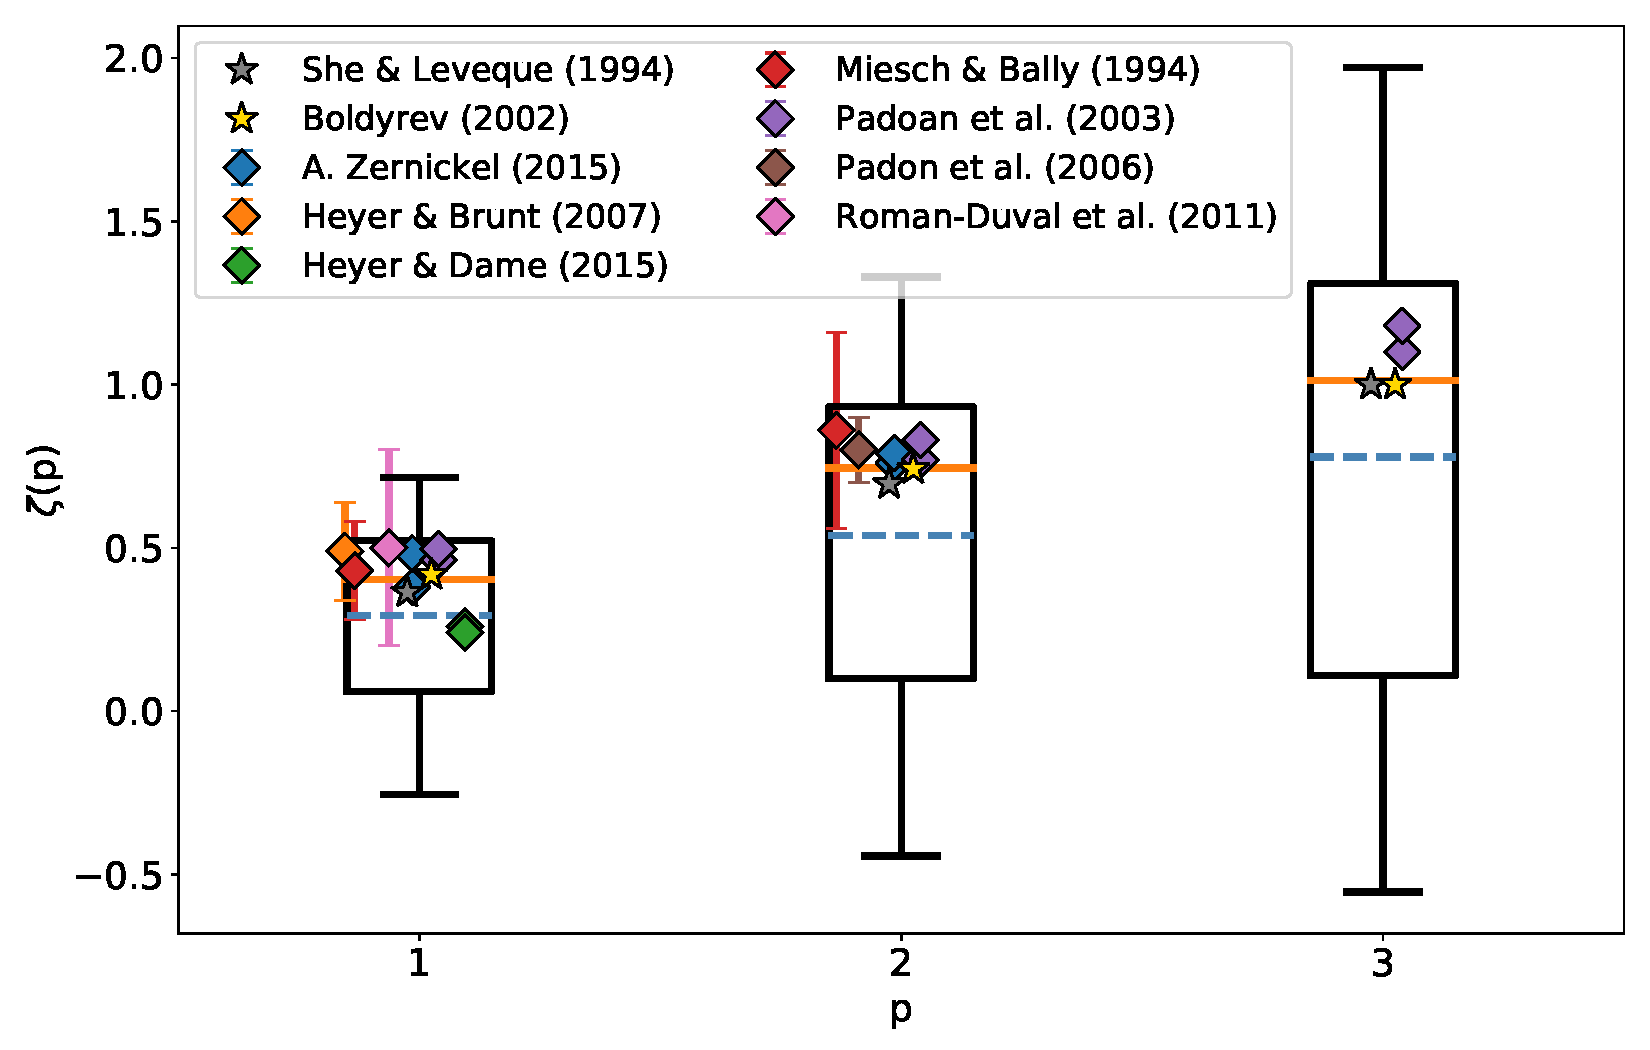
\includegraphics[width=0.49\textwidth]{compare_observations.pdf}
	\caption{Summary of measurements of $\zeta$ (\textit{abscissas}) and $Z$ (\textit{ordinates}) for orders $p=1$--3 (from \textit{left} to \textit{right}). The grey boxes represent the values presented in Sect.~\ref{results:normal}. The orange solid and blue dashed lines represent the average and median values of the distributions, respectively. The coloured star markers illustrate the predictions by \citet{She1994} and \citet{Boldyrev2002}. The coloured, circular markers summarise values found in the literature (see legend for precise references).
	}
	\label{pic:discussion:comp_observation}
\end{figure}


Compared to these measurements, the distributions of our results show a large scatter across the parameter space. 
However, we also see that there is a significant fraction of values in our models that are consistent with the observational findings. 
These measurements belong roughly to the evolutionary stages of the modelled clouds after having evolved for 1.5--4~Myr after the onset of self-gravity.
\citetalias{Chira2018} finds that the clouds consist of a highly hierarchical structure that is dominated by already fragmenting filaments at this point.
This means that the flows within the clouds experience a transition from cloud-scale dominated, through filament-dominated, to core-collapse driven motions; which is exactly what we observe in the VSFs, as well.
Consequently this suggests that the observed MCs, which show clear signs of embedded star formation activity, are in a similar stage where flows are dominated by the formation of hierarchical structures, (pre-/proto-)stellar cores or, in the case of NGC 6334, internal feedback.

We find that the interpretation of observational measurements is still difficult for several reasons:
\begin{enumerate}
\item We have already discussed in Sect.~\ref{discussion:1d} that the transformation from 3D to 1D VSFs is not trivial, in particular when the studied flows are not isotropic.
This is, for example, the case when the first structures (such as filaments or sheets) form, or the first cores collapse and accrete.
\item We have seen that interactions with SN shocks may trigger a preferred direction, that has the potential to strongly influence the measured 1D VSF.
Although the influence of shock fronts on VSFs is transient compared to the lifetime of the entire MC, it is still long enough to mimic a quasi-steady state in real observations.
Observing typical shock tracers, such as SiO, may help to identify these situations. 
\item We have neglected typical line-of-sight effects that may have a significant influence on the measurements of the local standard of rest velocity whose precision is crucial for this kind of study.
Our projections ignore optical depth effects, and reflect velocities all the way through the clouds, including high column density regions of dynamical collapse where motions are fast at small scales.  However, CO reaches optical depth of unity at relatively low column densities. This means that the observed VSFs will only reflect the motions of the surface layers of dense MCs.  
Therefore, single-tracer observations are not suitable for studying the dynamical structure of MCs. 
For a proper VSF analysis it would be advisable to use a variety of tracers to cover the different phases of the clouds, as well as to populate the statistics of lag distances more completely.
\item Only a small fraction of the listed observational studies in Table~\ref{tab:discussion:summary_obs} aimed to measure the VSFs of the respective objects directly.
In the majority of cases, the focus of the investigations was on the general budget of kinetic energy within the MC, as well as the question whether those clouds follow Larson's size-velocity relation (Eq.~[\ref{eq:larson}]).
It is unclear whether the difference between a relation of the lag distance of two particles and their relative line-of-sight velocity and the connection between the size of the entire MC and the velocity dispersion of the contained gas has always been considered.
\end{enumerate}

We recommend that both theorists and observers discuss in more detail how observational studies may use VSFs in the future.
From the theoretical point-of-view, full line radiative transfer calculations are required to better evaluate observational biases and simple projection effects.
This requires observations with a high spatial resolution of the respective MC for a wide range of lag scales and good statistics for fitting the scaling of VSF, as well as lines with well-defined line-of-sight velocities, ideally, optically thin lines of intermediate- and high-density tracers. 









\endinput

 	\section{Summary \& Conclusions}\label{conclusions}

In this paper, we analyse the turbulent structures of molecular clouds that have formed within 3D AMR FLASH simulations of the self-gravitating, magnetised, supernova-driven ISM by \citet{IbanezMejia2016}.
The main results are as follows.

\begin{itemize}
	\item The scaling of velocity structure functions (VSFs) is sensitive to both internal (gravitational contraction) and external (SN shocks, winds) driving sources of turbulence. Applied on simulated data, the time evolution of the scaling exponent, $\zeta$, can reveal which driving mechanism dominates the turbulence of an entire molecular cloud. The self-similarity parameter, $Z$, though, is not directly sensitive to gravitational contraction. Yet, it can be used as observational tracer as it significantly reacts to SNe and winds.
	\item As long as the molecular cloud is not affected by a shock, $Z$ is in good agreement with predicted values for supersonic flows. This makes it a fine probe for the properties of dominant turbulent modes, such as the geometry, and their evolution in the context with the evolution of the cloud. 
	\item We test the influence of Jeans refinement on the VSFs. We find that the absolute amount of kinetic energy does not influence the evolution of $\zeta$ and $Z$, as long as the power spectrum is properly resembled, or similarly resembled by the compared samples.
	\item We see that the behaviour of the VSFs can be tracked with similar results based on 3D (i.e., from simulated data) and 1D (i.e., from observational data) velocity information, as long as there is no dominating flow driving the gas into a direction perpendicular to the line of sight. In the general case of a fully developed turbulent field, both $\zeta$ and $Z$ evolve similarly in both scenarios, even though the actual values might not be in good agreement.
	\item We test the influence of introducing a density threshold on the VSFs. We see both quantitative and qualitative differences. The VSFs that based on the unfiltered data are much steeper than the cloud-only VSFs and do not reflect any interaction with any of the driving sources, including SN shocks. The measured $Z$ values are constant in time and and for all clouds. This means that the turbulence we examine in this sub-project reflects the ISM in our entire galactic-scale simulations. The values of $Z$ are slightly below the value predicted for a filamentary flow by \citet{She1994}. We conclude that the turbulence in the modelled ISM consists of vortices that are similar to filamentary flows, yet with a ratio of average length scale of the two moments being more equal to unity than in the filamentary case.
	\item We investigate the influence of defining the VSF with and without taking density weighting into account. We see that the qualitative behaviour is traced by both approaches. Yet, the scaling of the non-weighted VSF is always positive and evolve flatter than they do for the density-weighted VSF. This means that non-weighted VSFs that are based on smoothed density distributions are biased against large scale motions and may not reveal the entire distribution of turbulent power within a molecular cloud. 
\end{itemize}

Our analysis shows that VSFs are fine tools for examining the driving source of turbulence within molecular clouds.
Therefore, we recommend its usage in future studies of molecular clouds.
However, studies that utilise VSFs need to precisely review the assumptions and parameters they imply in their analysis as those can have a significant influence on the out-coming results.

For the simulated clouds, the VSFs illustrate that gravitational contraction dominates the evolution of the clouds, with short periods within which SN shock waves accelerate the turbulent powers on all scales. 
However, it requires further studies to verify this to be the common fragment formation scenario. 
In particular, a higher Jeans length refinement is needed to resolve the velocity structures on scales of individual grid cells (0.1~pc in this case) better.
This is crucial for following the local behaviour of the gas as neither the average behaviour of the filaments nor the dominant turbulence driving source of the entire molecular clouds mirror the underling flow patterns of the gas that is related to fragmentation and the formation of future star formation activity. 



\endinput

 
 	\begin{acknowledgements}
 		R-AC acknowledges the support ESO and its Studentship Programme provided.
         M-MML received support from US NSF grant AST11-09395 and thanks the A. von Humboldt-Stiftung for support.  
         JCI-M was additionally supported by the DFG Priority Programme 157.
 	\end{acknowledgements}

 	\bibliographystyle{aa} % style aa.bst
 	\bibliography{ref}

% 	\appendix
% 		\input{a_filfinder}
%         %\onecolumn
%         %\thispagestyle{headings}
%     	%\input{a_figures}
        
        
\end{document}
